\documentclass[12pt,a4paper]{article}

\usepackage[utf8]{inputenc}
\usepackage[T1]{fontenc}
\usepackage[english]{babel}
\usepackage{geometry}
\geometry{margin=2.5cm}

\usepackage{graphicx}
\usepackage{booktabs}
\usepackage{tabularx}
\usepackage{multirow}
\usepackage{float}
\usepackage{amsmath}
\usepackage{hyperref}
\usepackage{caption}
\usepackage{subcaption}
\usepackage{xcolor}
\usepackage{pgfplots}
\pgfplotsset{compat=1.18}
\usepackage{pgfplotstable}
\usepackage{listings}
\usepackage{parskip}

\lstset{
  basicstyle=\ttfamily\footnotesize,
  breaklines=true,
  frame=single,
  backgroundcolor=\color{gray!8},
  keywordstyle=\color{blue},
  commentstyle=\color{gray},
}

\hypersetup{colorlinks=true, linkcolor=blue, urlcolor=blue, citecolor=blue}

% ─────────────────────────────────────────────────────────────────────────────
\title{\textbf{Big Data Storage and Retrieval}\\
       \large Assignment 2: Multi-Model Database Benchmarking\\[0.5em]
       \normalsize E-Commerce Event Dataset}
\author{Ivan Alpatov}
\date{\today}

\begin{document}
\maketitle
\tableofcontents
\newpage

% ═════════════════════════════════════════════════════════════════════════════
\section{Abstract}
% ═════════════════════════════════════════════════════════════════════════════

This report presents the design, implementation, and benchmarking of four database
models built over a real-world e-commerce event dataset. The dataset records
user interactions (views, cart additions, purchases) with products, alongside
marketing campaign messages and social network friendships.

Four storage backends were implemented and compared:
\begin{itemize}
  \item \textbf{PostgreSQL 3NF} --- fully normalised relational model,
  \item \textbf{PostgreSQL Own} --- a denormalised variant optimised for event queries,
  \item \textbf{MongoDB} --- document-oriented store with embedded product metadata,
  \item \textbf{Memgraph} --- property graph model for relationship-heavy queries.
\end{itemize}

Three analytical queries were executed five times on each backend after a
warm-up run, and their execution times were recorded. The key finding is that
PostgreSQL significantly outperforms MongoDB and Memgraph for all tested
workloads, while the graph model excels at traversal queries (Q1b) but
struggles with aggregation-heavy recommendation tasks (Q2, Q3).

% ═════════════════════════════════════════════════════════════════════════════
\section{Environment and Setup}
% ═════════════════════════════════════════════════════════════════════════════

\subsection{Hardware}
\begin{table}[H]
\centering
\begin{tabular}{ll}
\toprule
\textbf{Component} & \textbf{Specification} \\
\midrule
OS        & Windows 10 Pro (build 19045) \\
CPU       & 11th Gen Intel Core i5-1135G7 \\
CPU Clock & 2.40 GHz base (4 cores / 8 logical processors) \\
RAM       & 16 GB \\
Platform  & ASUS VivoBook X513EA (laptop) \\
\bottomrule
\end{tabular}
\caption{Test machine specifications}
\end{table}

\subsection{Software}
\begin{table}[H]
\centering
\begin{tabular}{lll}
\toprule
\textbf{Software} & \textbf{Version} & \textbf{Deployment} \\
\midrule
PostgreSQL  & 15              & Docker container \\
MongoDB     & 7.0             & Docker container \\
Memgraph    & 2.x (MAGE)      & Docker container \\
Python      & 3.13            & Local (Windows) \\
pandas      & 2.x             & pip \\
\bottomrule
\end{tabular}
\caption{Software stack}
\end{table}

All three databases ran inside Docker containers on the same host machine (no
virtual machines). Python scripts connected to each container over \texttt{localhost}
using standard drivers (\texttt{psycopg2}, \texttt{pymongo}, \texttt{neo4j}).

% ═════════════════════════════════════════════════════════════════════════════
\section{Data Modelling}
% ═════════════════════════════════════════════════════════════════════════════

\subsection{Dataset Overview}

The source dataset is a CSV export of an e-commerce platform containing:
\begin{itemize}
  \item \textbf{Events}: user interaction records (view, cart, purchase) each
        linked to a product, a category, and optionally a brand and price.
  \item \textbf{Messages}: marketing campaign messages sent to clients,
        with flags \texttt{is\_opened}, \texttt{is\_clicked}, \texttt{is\_purchased}.
  \item \textbf{Campaigns}: metadata (type, channel) for each campaign.
  \item \textbf{Clients / Users}: registered users who can receive messages
        and generate events.
  \item \textbf{Friendships}: undirected social graph between users.
\end{itemize}

\subsection{SCD Type 2 Surrogate Keys}

A key data-quality challenge was that the same \texttt{product\_id} occasionally
appeared with different \texttt{category\_id} or \texttt{category\_code} values
across events — products that were re-categorised over time.
A naïve model keeping only one canonical category per product would
silently resolve every historical event to the \emph{last-known} category,
distorting category-level aggregations.

To preserve historical accuracy, \textbf{SCD Type 2 surrogate keys} were
introduced during pre-processing (\texttt{clean\_data.py}):

\begin{itemize}
  \item \textbf{\texttt{category\_sk}}: unique per \texttt{(category\_id, category\_code)} pair.
        Two rows with the same \texttt{category\_id} but different
        \texttt{category\_code} receive different surrogate keys.
  \item \textbf{\texttt{product\_sk}}: unique per
        \texttt{(product\_id, category\_id, category\_code)} triple.
        One physical product that appeared in two categories becomes two
        distinct surrogate-key versions.
\end{itemize}

Each event row in \texttt{events.csv} is enriched with the \texttt{product\_sk}
that was current at event time, enabling every downstream model to resolve the
correct historical category version via a single key lookup.

\begin{figure}[H]
  \centering
  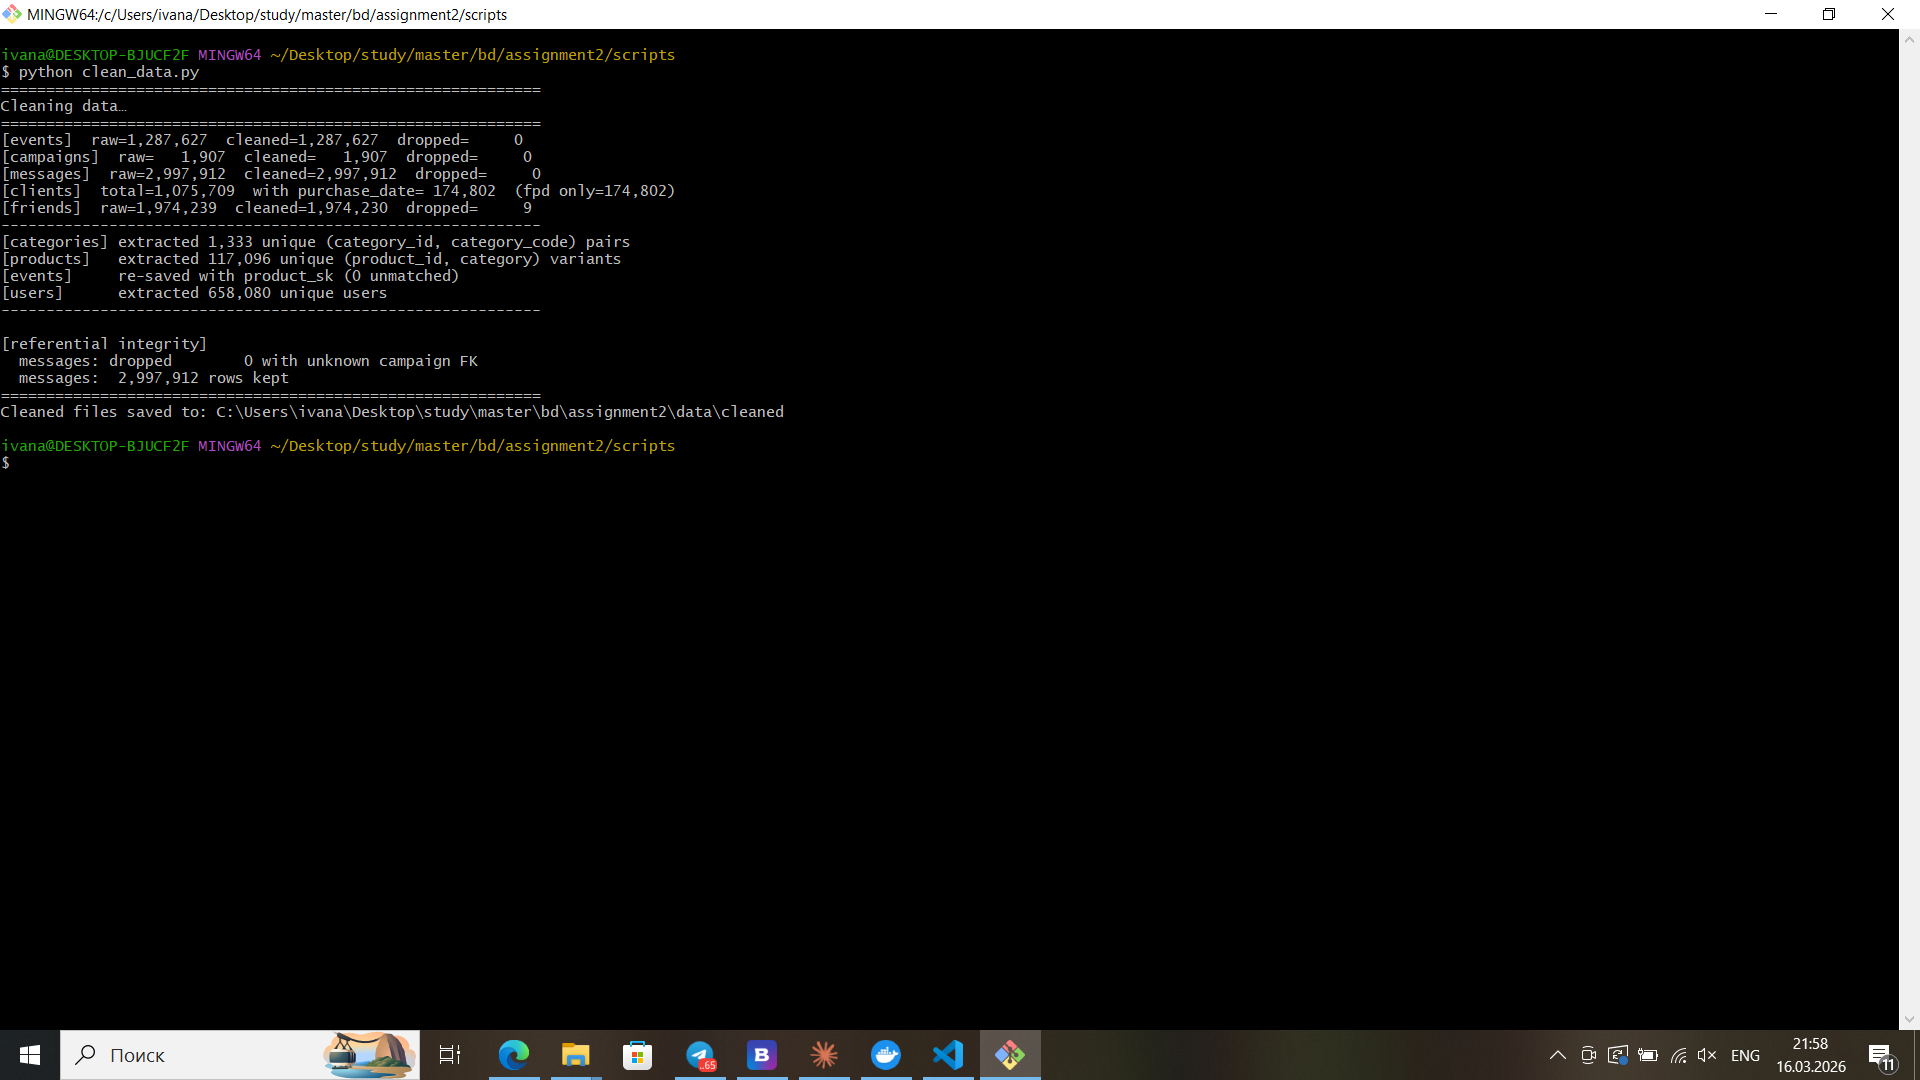
\includegraphics[width=\linewidth]{screenshots/clean_data.png}
  \caption{Pre-processing pipeline output (\texttt{clean\_data.py})}
\end{figure}

\subsection{PostgreSQL 3NF Model}

The 3NF schema enforces full normalisation:

\begin{verbatim}
categories (category_sk PK, category_id, category_code)
products   (product_sk PK, product_id, category_sk FK, brand, last_known_price)
events     (event_id PK, user_id, product_sk FK, event_type, event_time, price)
clients    (client_id PK, user_id FK, ...)
campaigns  (campaign_id PK, campaign_type, channel)
messages   (message_id PK, client_id FK, campaign_id FK, ...)
friendships(user_id_1 FK, user_id_2 FK)
\end{verbatim}

No data is duplicated. Every join traverses explicit foreign keys. The
\texttt{events} table references only \texttt{product\_sk}; the category is
always resolved through the chain
\texttt{events} $\to$ \texttt{products} $\to$ \texttt{categories}.

\begin{figure}[H]
  \centering
  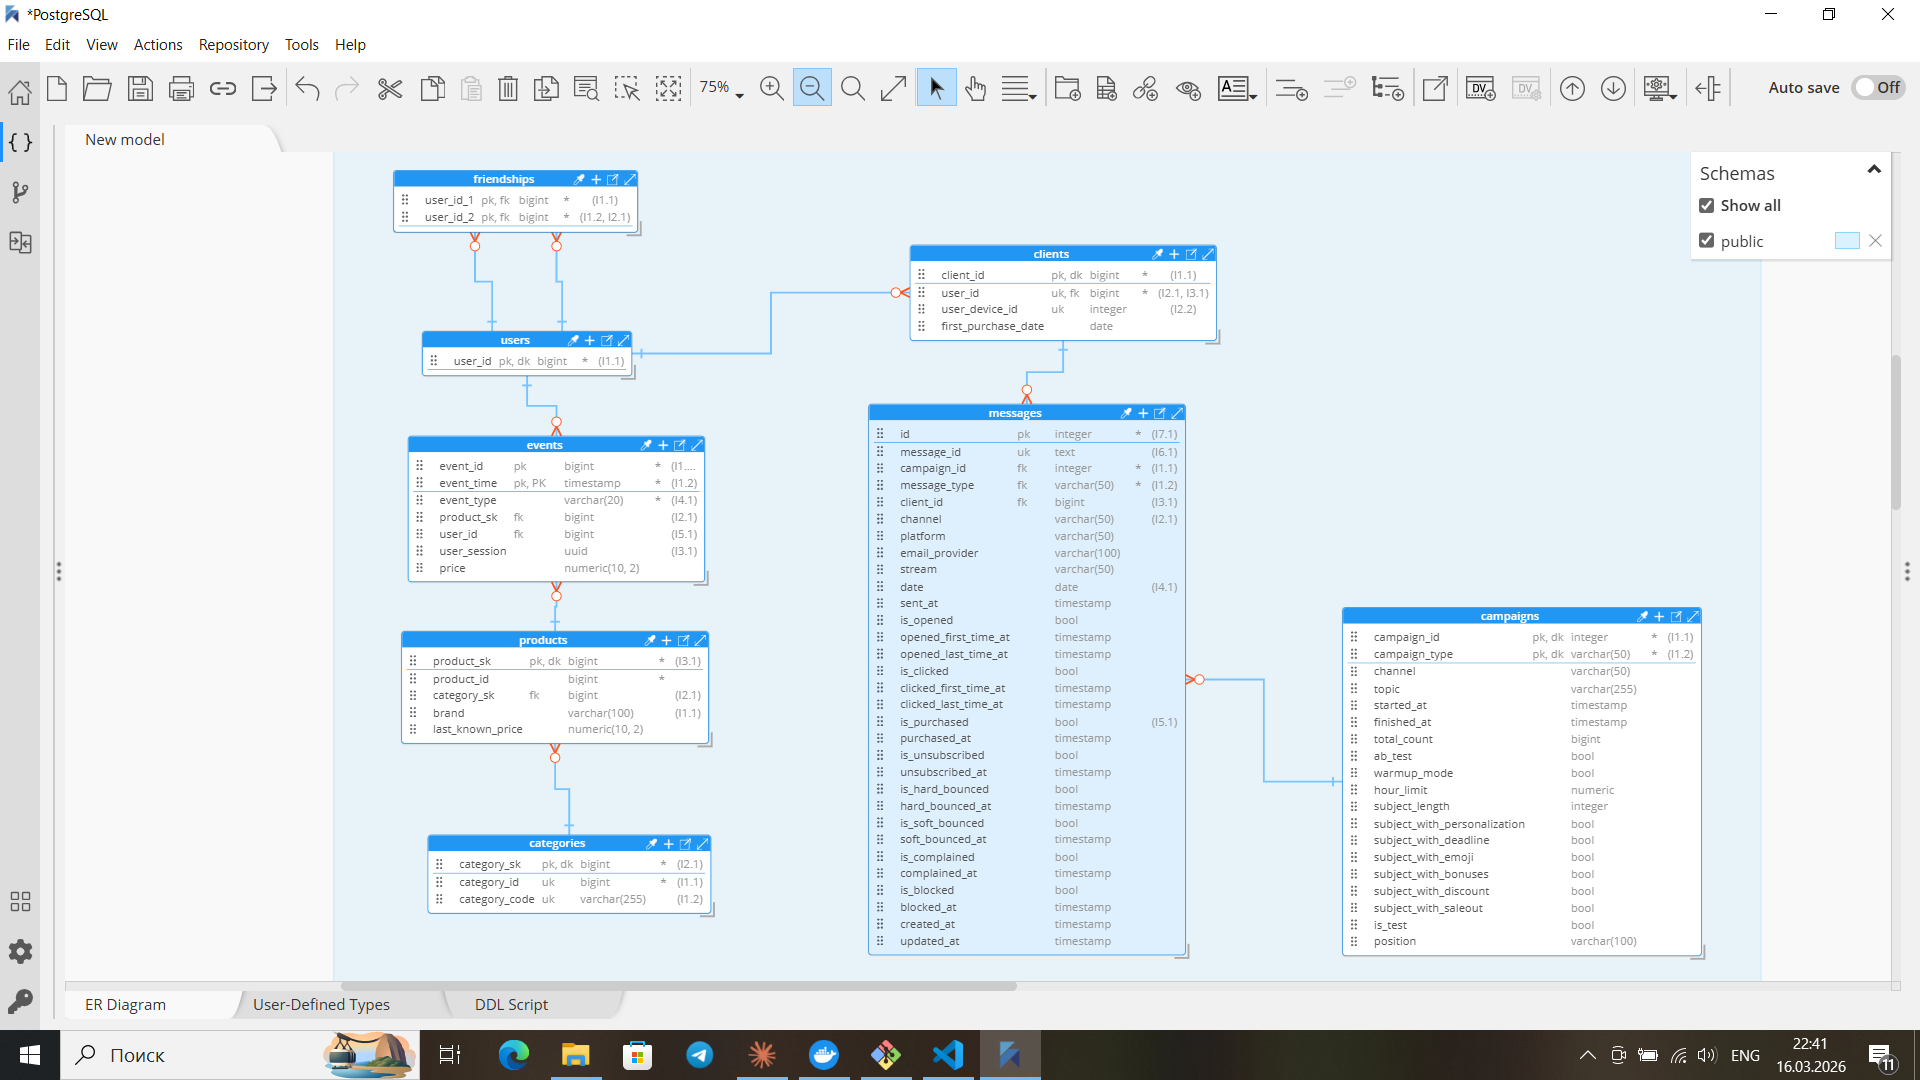
\includegraphics[width=\linewidth]{screenshots/PostgreSQL.png}
  \caption{PostgreSQL 3NF schema}
\end{figure}

\begin{figure}[H]
  \centering
  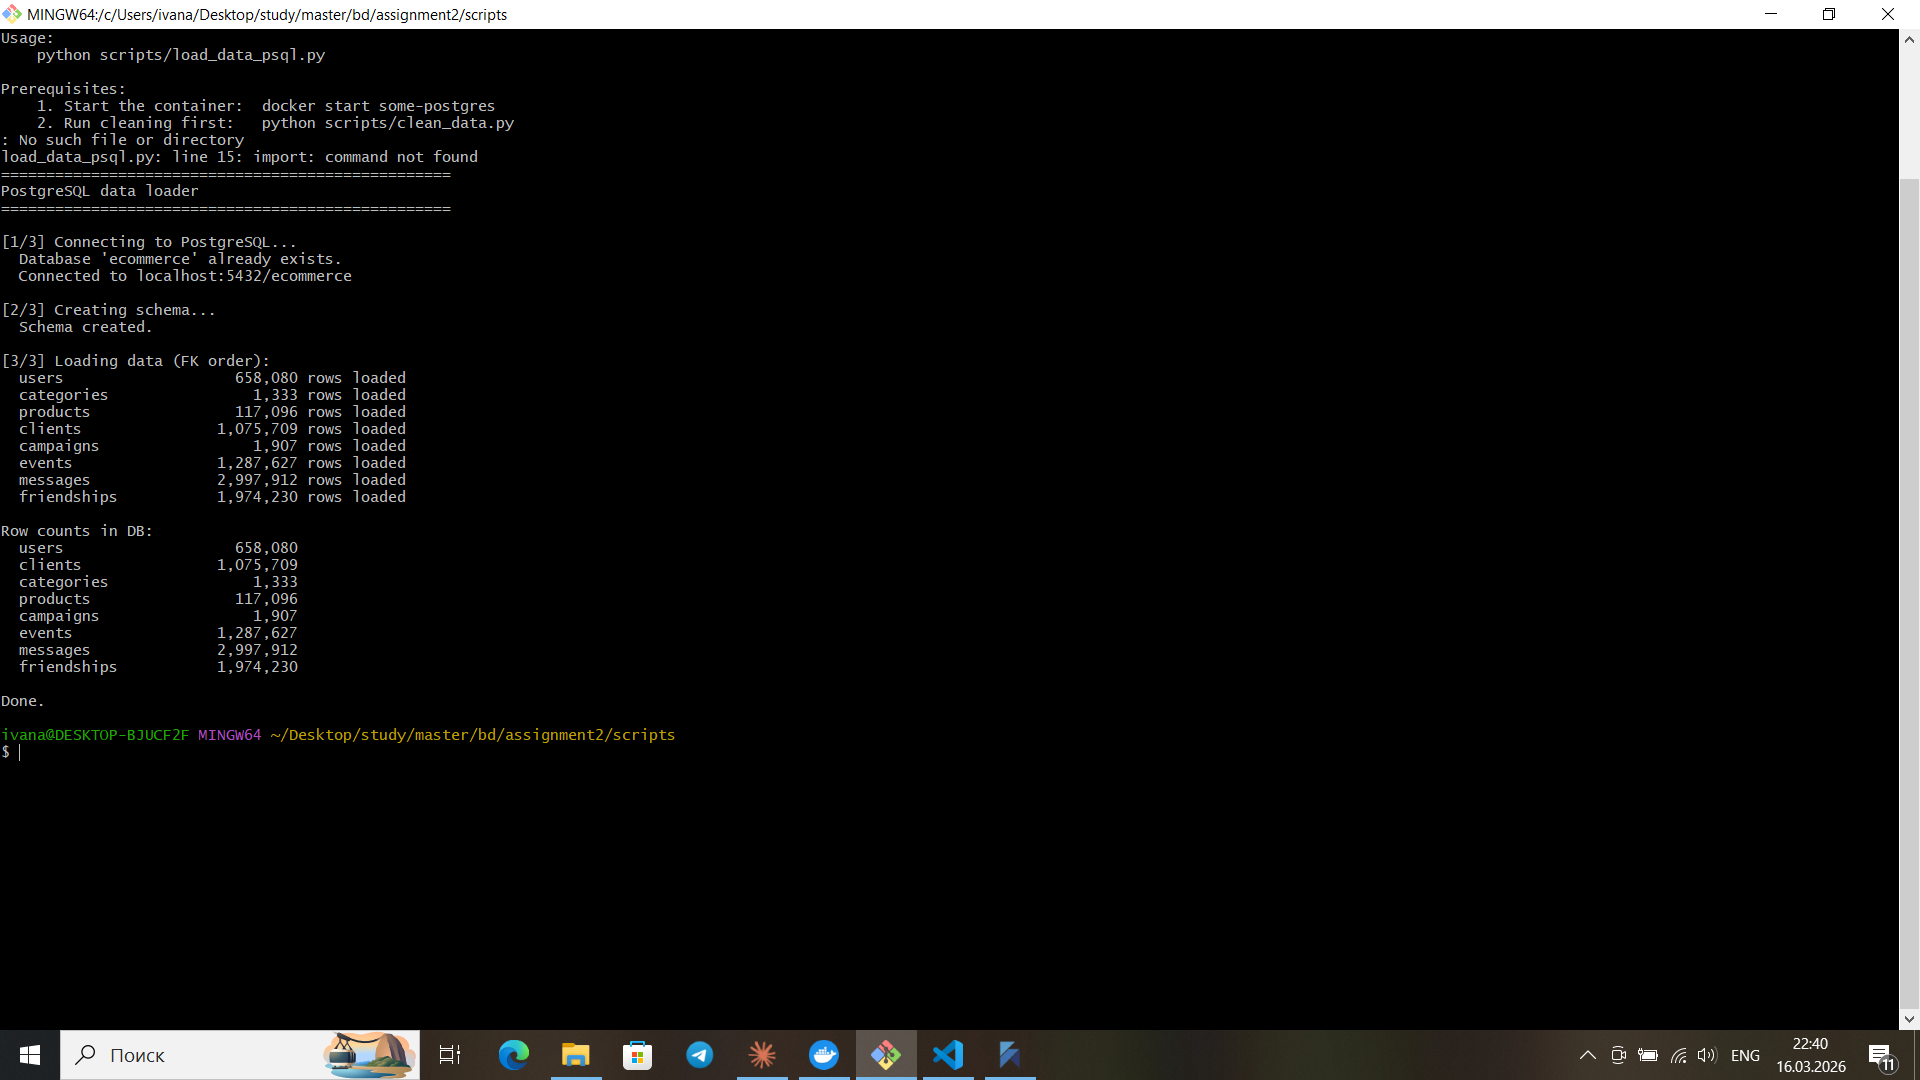
\includegraphics[width=\linewidth]{screenshots/load_data_psql.png}
  \caption{PostgreSQL 3NF data loading}
\end{figure}

\subsection{PostgreSQL Own (Denormalised) Model}

The \emph{own} model trades storage efficiency for query speed by
\textbf{inlining category attributes directly into the events table}:

\begin{verbatim}
events (event_id PK, user_id, product_sk FK, category_sk FK,
        product_id, brand, category_id, category_code,
        event_type, event_time, price)
\end{verbatim}

\textbf{Advantages:}
\begin{itemize}
  \item Q2 (recommendations) and Q3 (search) avoid joins to
        \texttt{products} and \texttt{categories} --- all needed columns
        are already in \texttt{events}.
  \item Analytical aggregations group directly on inline columns.
\end{itemize}

\textbf{Disadvantages:}
\begin{itemize}
  \item Update anomalies: changing a category name requires updating
        every affected event row.
  \item Higher storage footprint due to repeated string values.
\end{itemize}

The surrogate keys (\texttt{product\_sk}, \texttt{category\_sk}) are still
maintained so that historical accuracy is preserved even in the denormalised
form.

\begin{figure}[H]
  \centering
  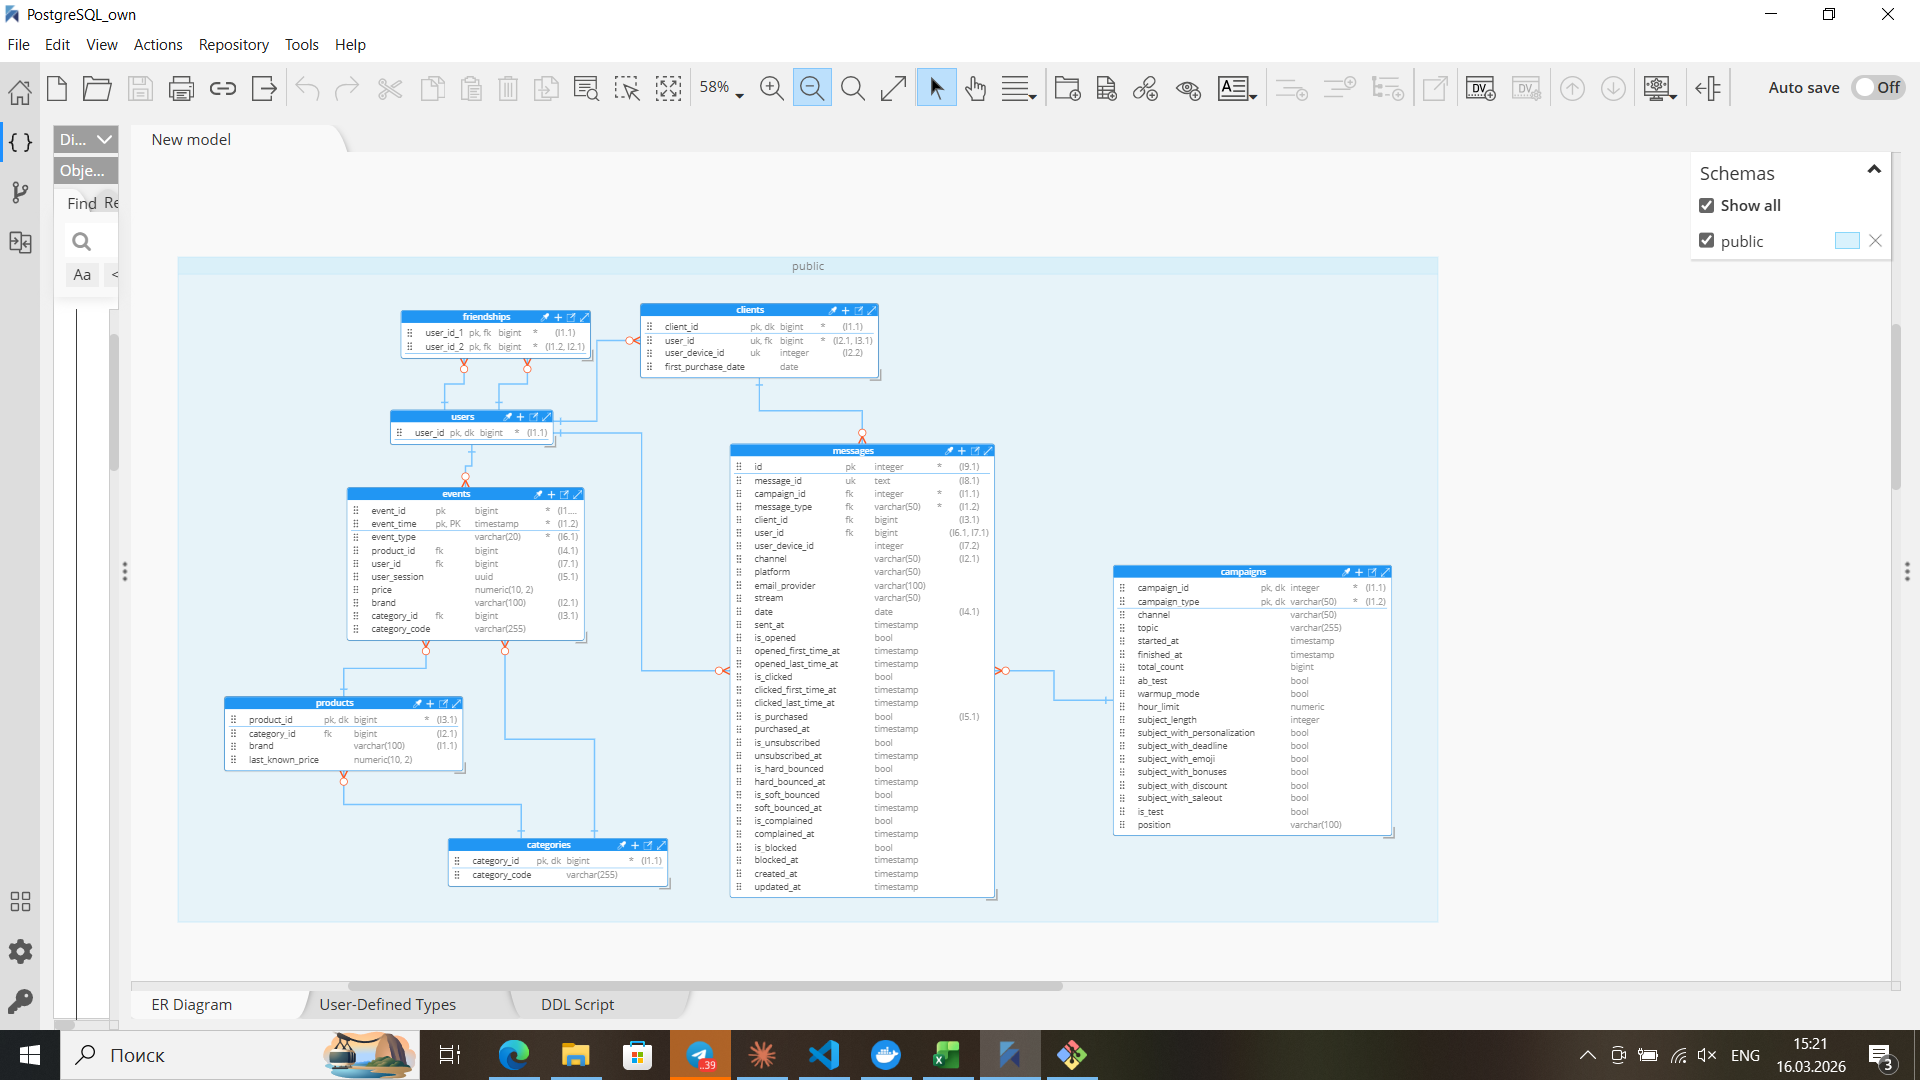
\includegraphics[width=\linewidth]{screenshots/PostgreSQL_own.png}
  \caption{PostgreSQL Own (denormalised) schema}
\end{figure}

\begin{figure}[H]
  \centering
  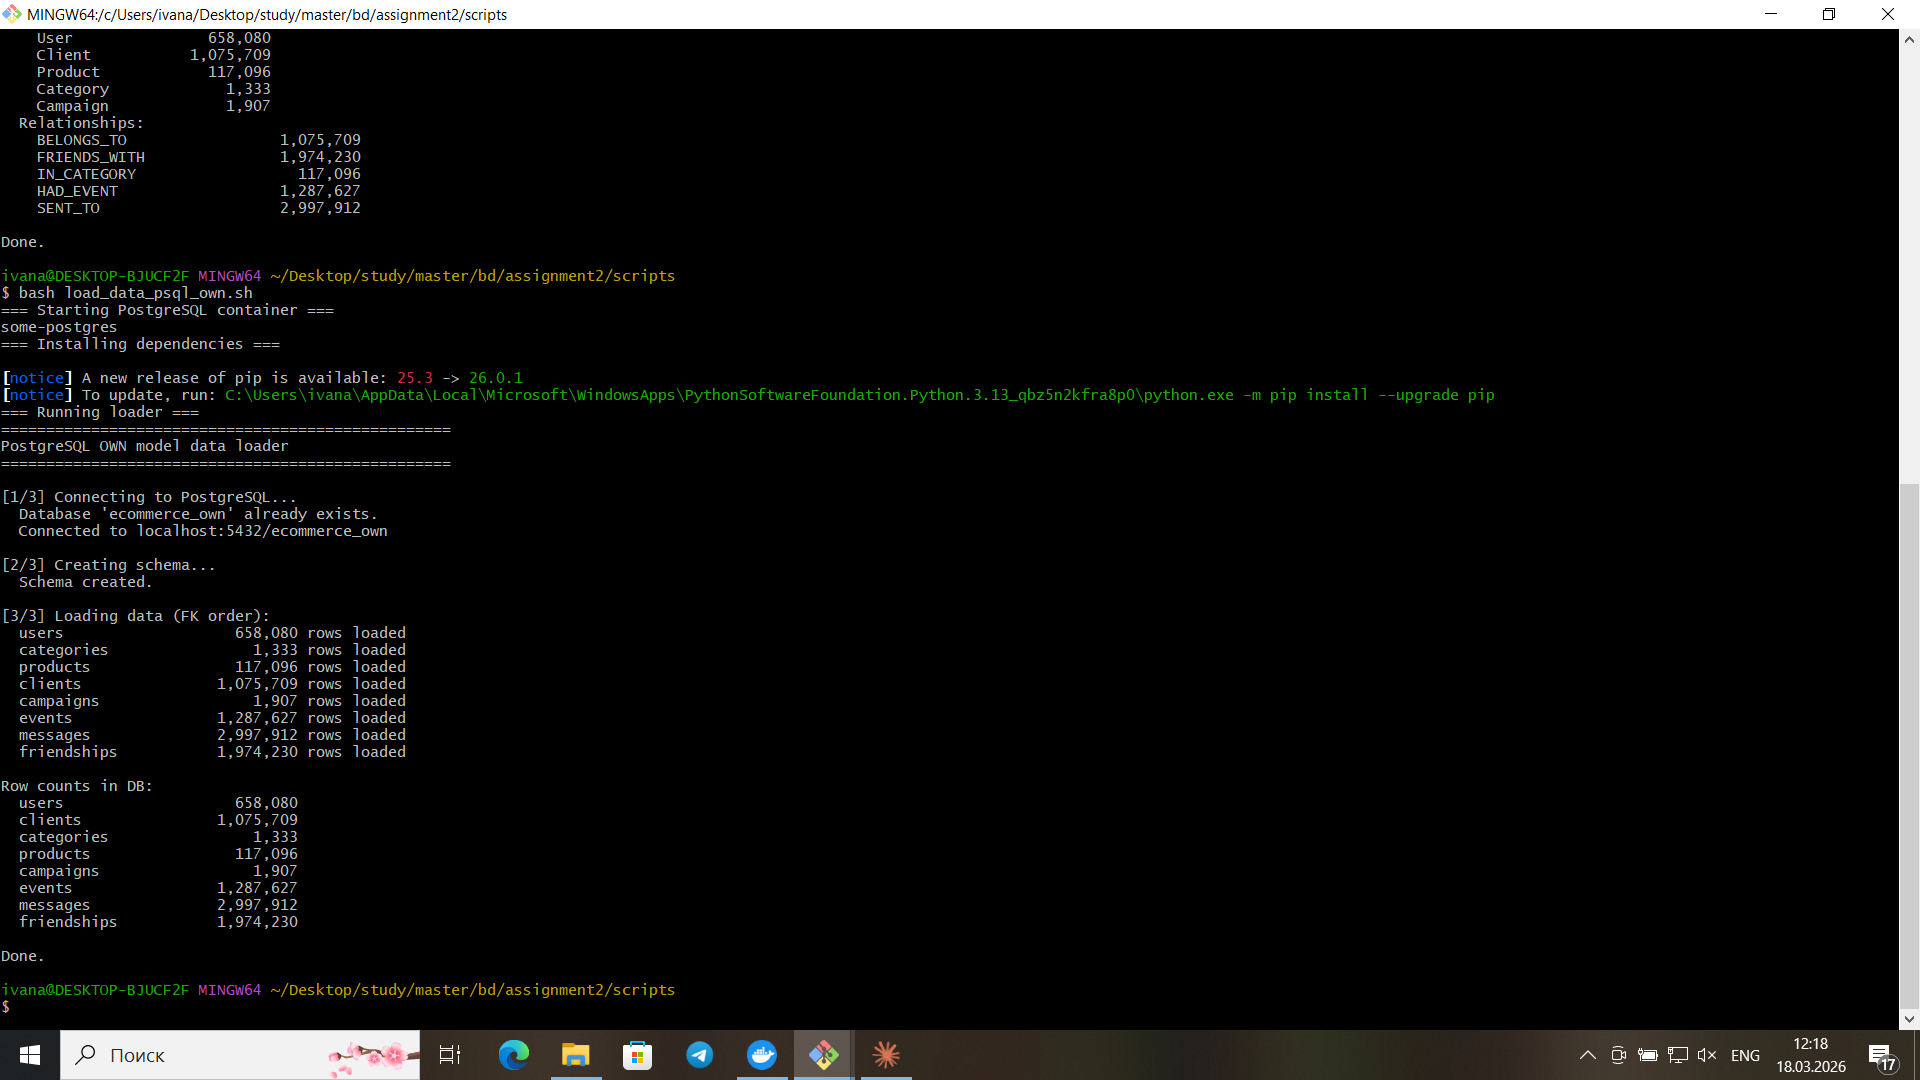
\includegraphics[width=\linewidth]{screenshots/load_data_psql_own.png}
  \caption{PostgreSQL Own data loading}
\end{figure}

\subsection{MongoDB Document Model}

MongoDB stores each entity type as a separate collection.
Products are stored with an \textbf{embedded category sub-document}:

\begin{lstlisting}[language={}]
// products collection
{
  "_id": <product_sk>,
  "product_id": 1004856,
  "brand": "samsung",
  "last_known_price": 128.42,
  "category": {
    "category_id": 1064,
    "category_code": "construction.tools.light"
  }
}
\end{lstlisting}

The \texttt{events} collection stores flat documents referencing
\texttt{product\_sk}. Events are \emph{not} embedded inside user documents
because the event volume (millions of rows) would exceed MongoDB's 16 MB
per-document limit and make targeted updates impractical.
Similarly, messages are stored separately from companies (campaigns) to avoid
unbounded array growth.

\begin{figure}[H]
  \centering
  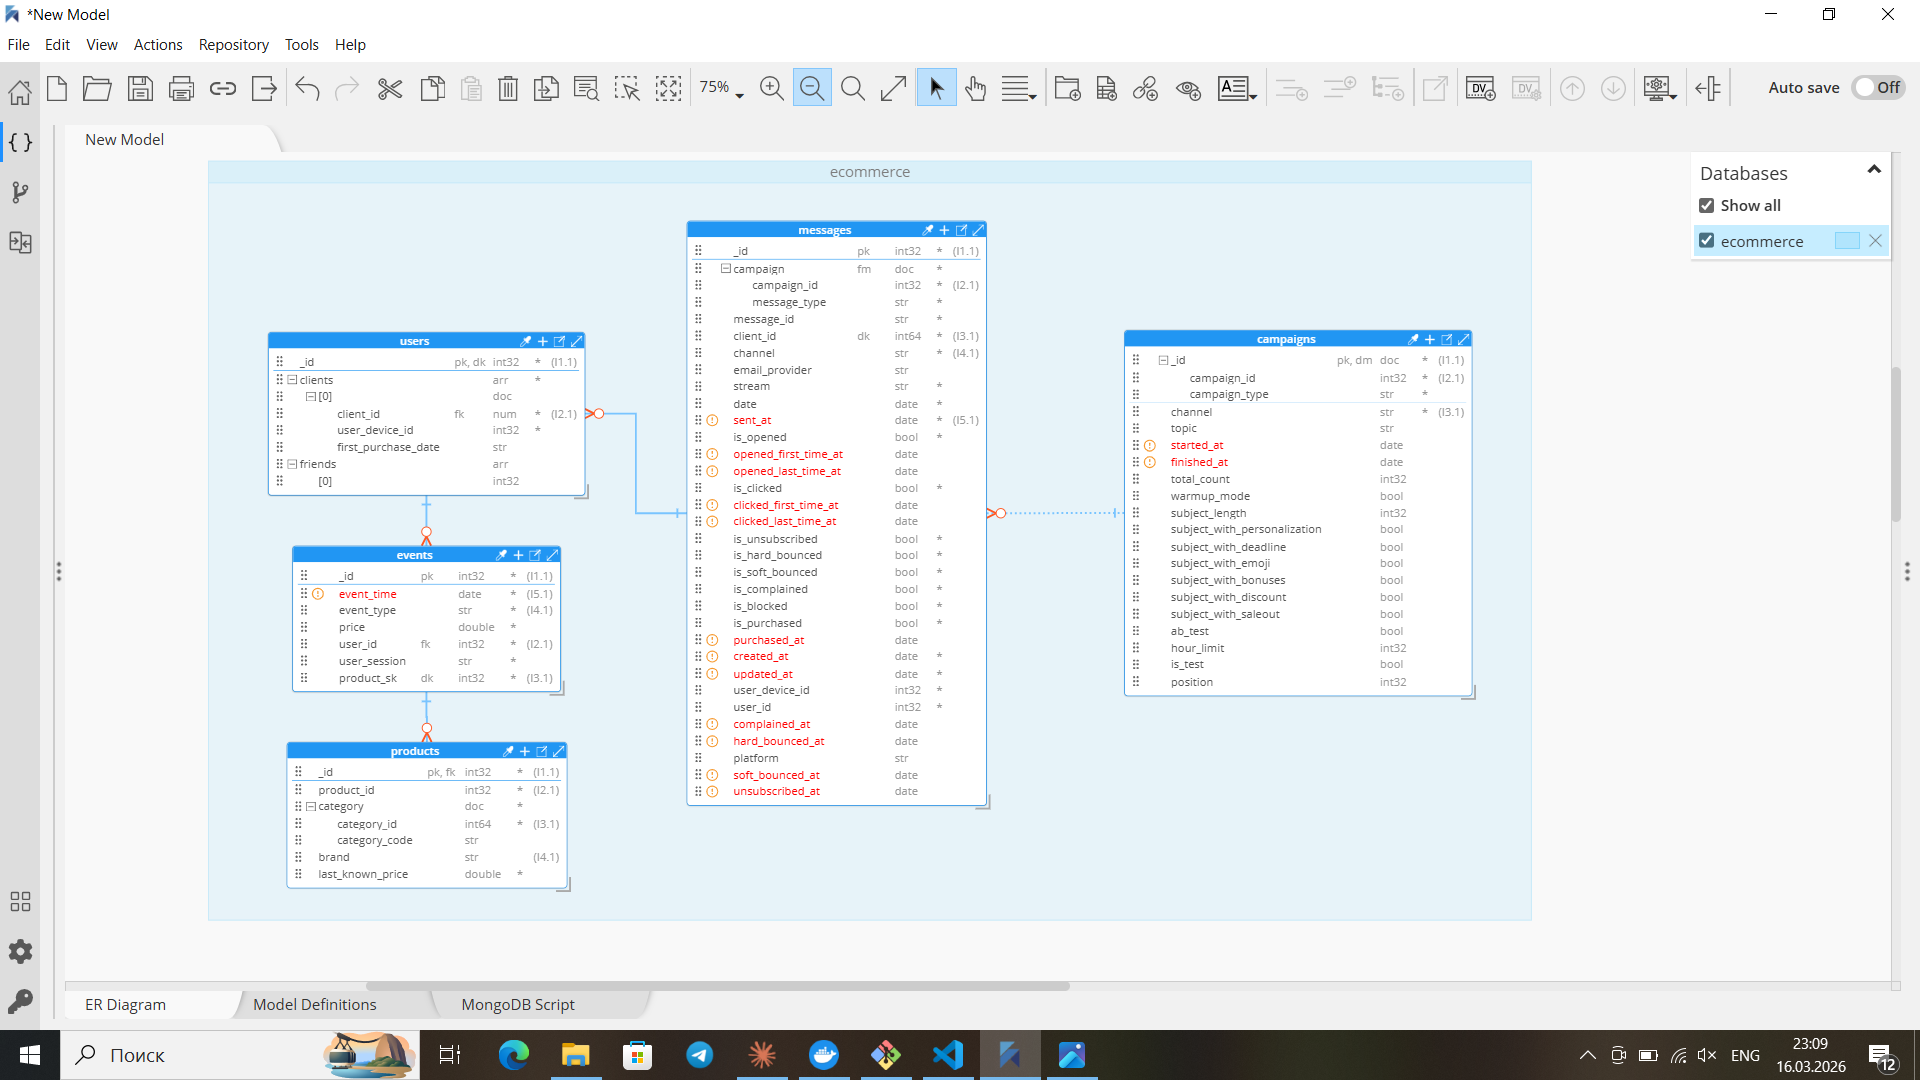
\includegraphics[width=\linewidth]{screenshots/MongoDB.png}
  \caption{MongoDB collection design}
\end{figure}

\begin{figure}[H]
  \centering
  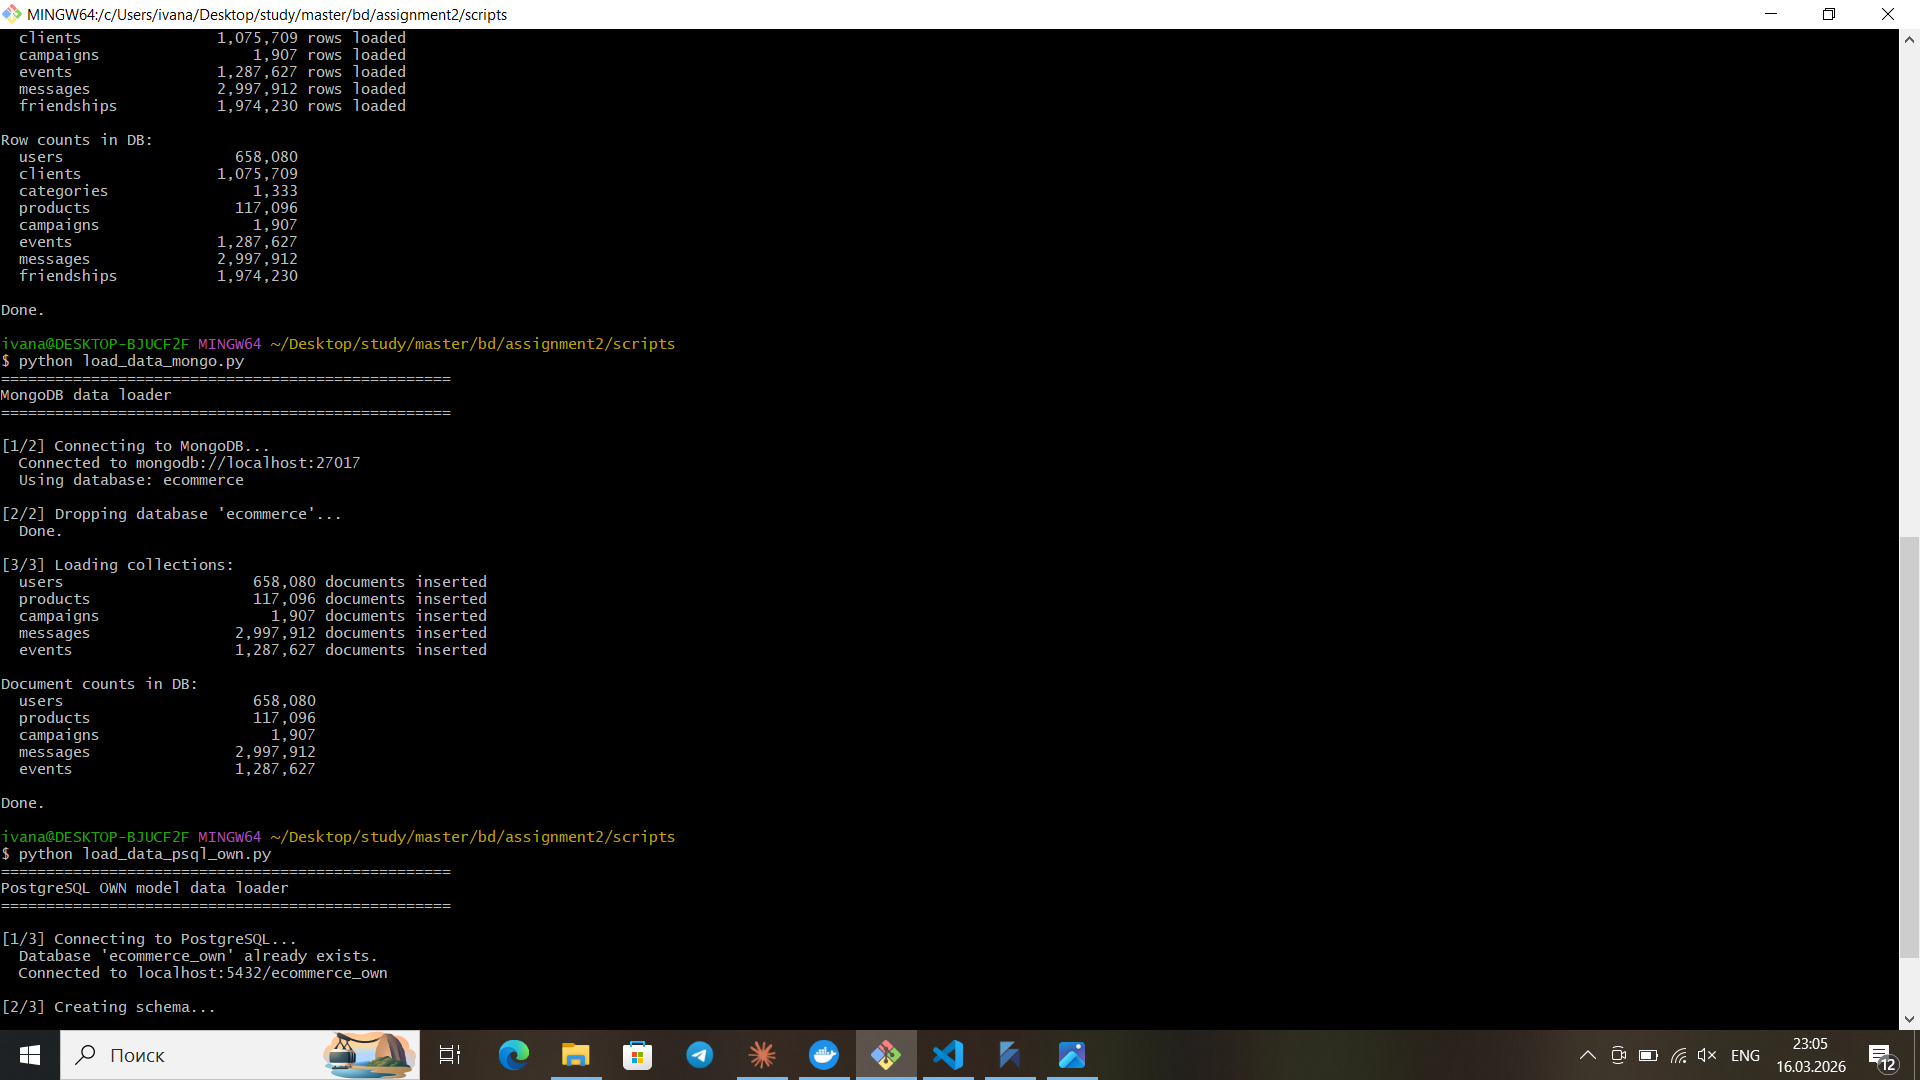
\includegraphics[width=\linewidth]{screenshots/load_data_mongo.png}
  \caption{MongoDB data loading}
\end{figure}

\subsection{Memgraph Property Graph Model}

The graph schema uses one node label per entity and typed relationships:

\begin{verbatim}
(:User)-[:HAD_EVENT {event_type, price, event_time}]->(:Product)
(:Product)-[:IN_CATEGORY]->(:Category)
(:User)-[:IS_CLIENT]->(:Client)
(:Client)-[:RECEIVED]->(:Message)-[:PART_OF]->(:Campaign)
(:User)-[:FRIENDS_WITH]->(:User)
\end{verbatim}

\textbf{Key design decisions:}
\begin{itemize}
  \item One \texttt{Product} node per \texttt{product\_sk} (not per
        \texttt{product\_id}). This preserves the historical category version
        at the graph-structure level: two re-categorisations of the same
        physical product become two separate nodes connected to their
        respective \texttt{Category} nodes.
  \item Unique constraints are placed on \texttt{product\_sk} and
        \texttt{category\_sk}, not on \texttt{product\_id} /
        \texttt{category\_id}, for the same reason.
  \item The \texttt{FRIENDS\_WITH} relationship is stored in both directions
        to make undirected traversal efficient.
\end{itemize}

\begin{figure}[H]
  \centering
  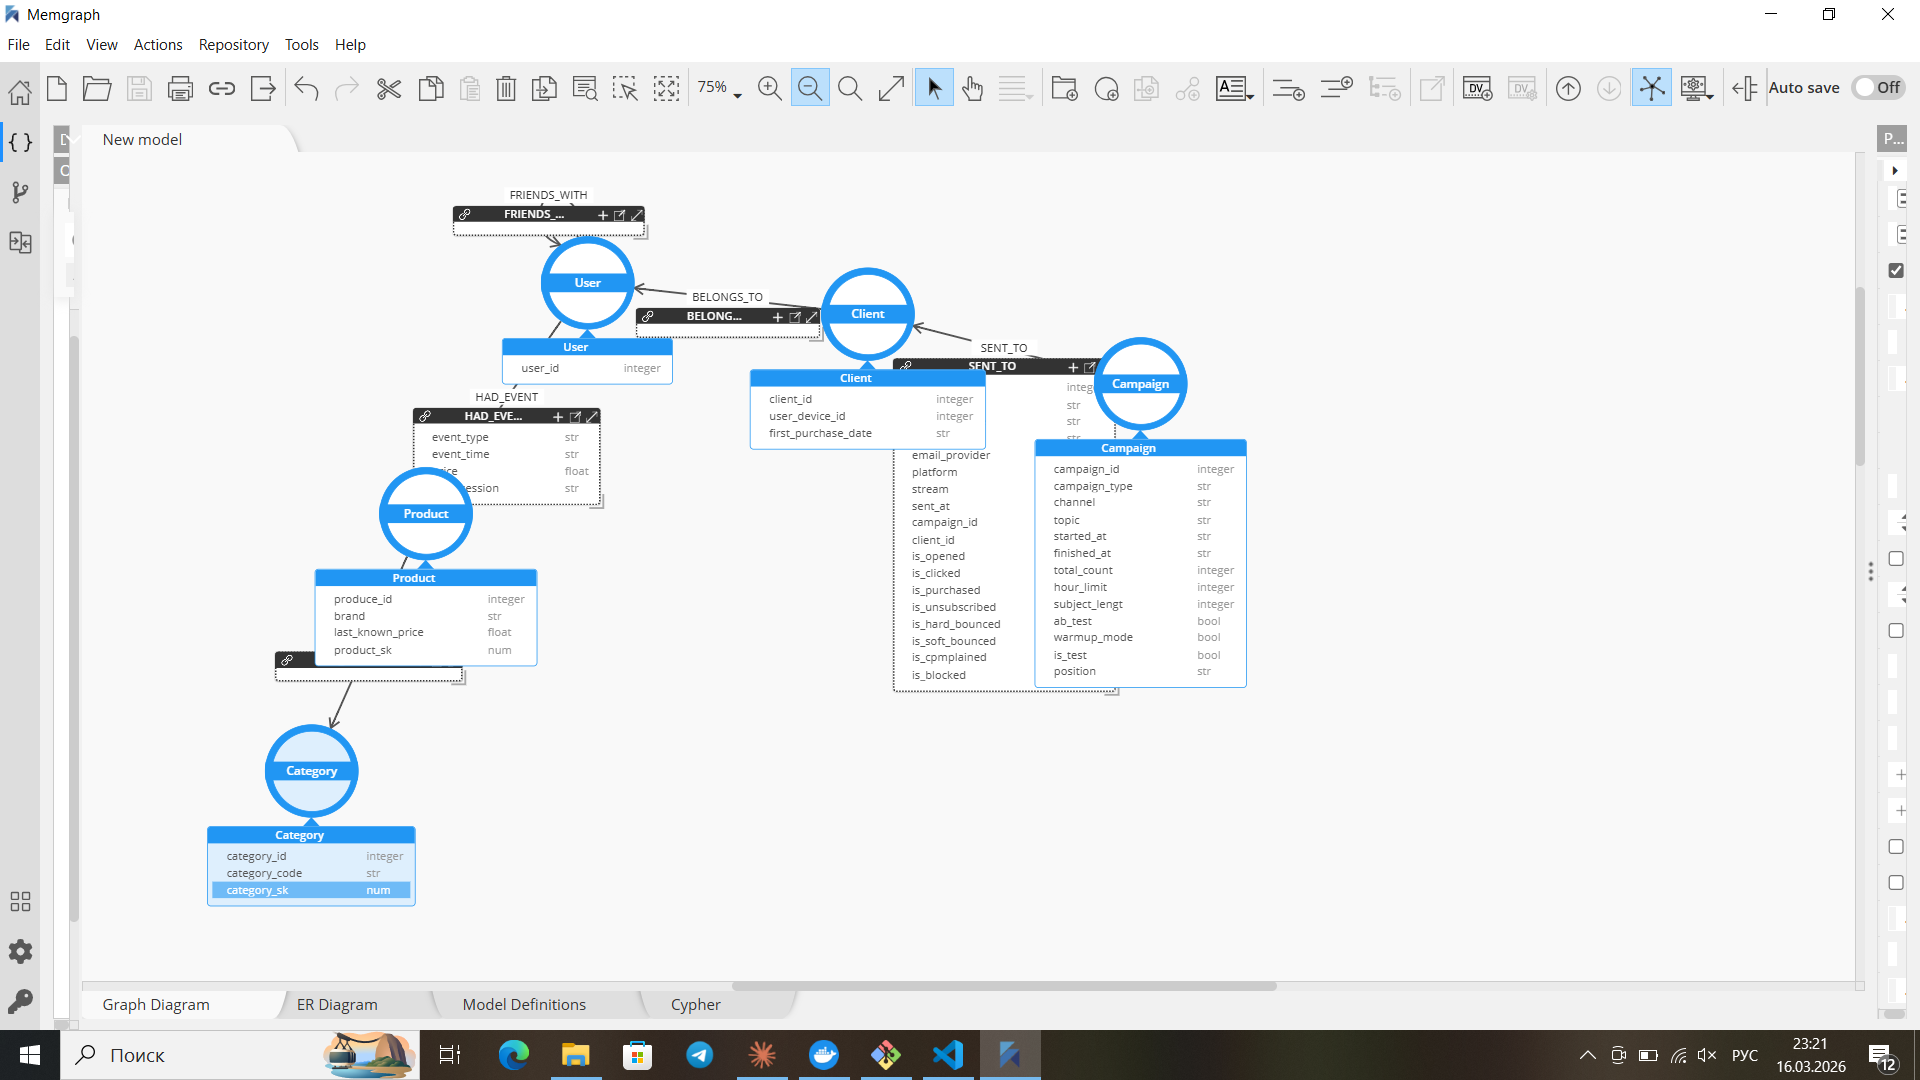
\includegraphics[width=\linewidth]{screenshots/Memgraph.png}
  \caption{Memgraph property graph schema}
\end{figure}

\begin{figure}[H]
  \centering
  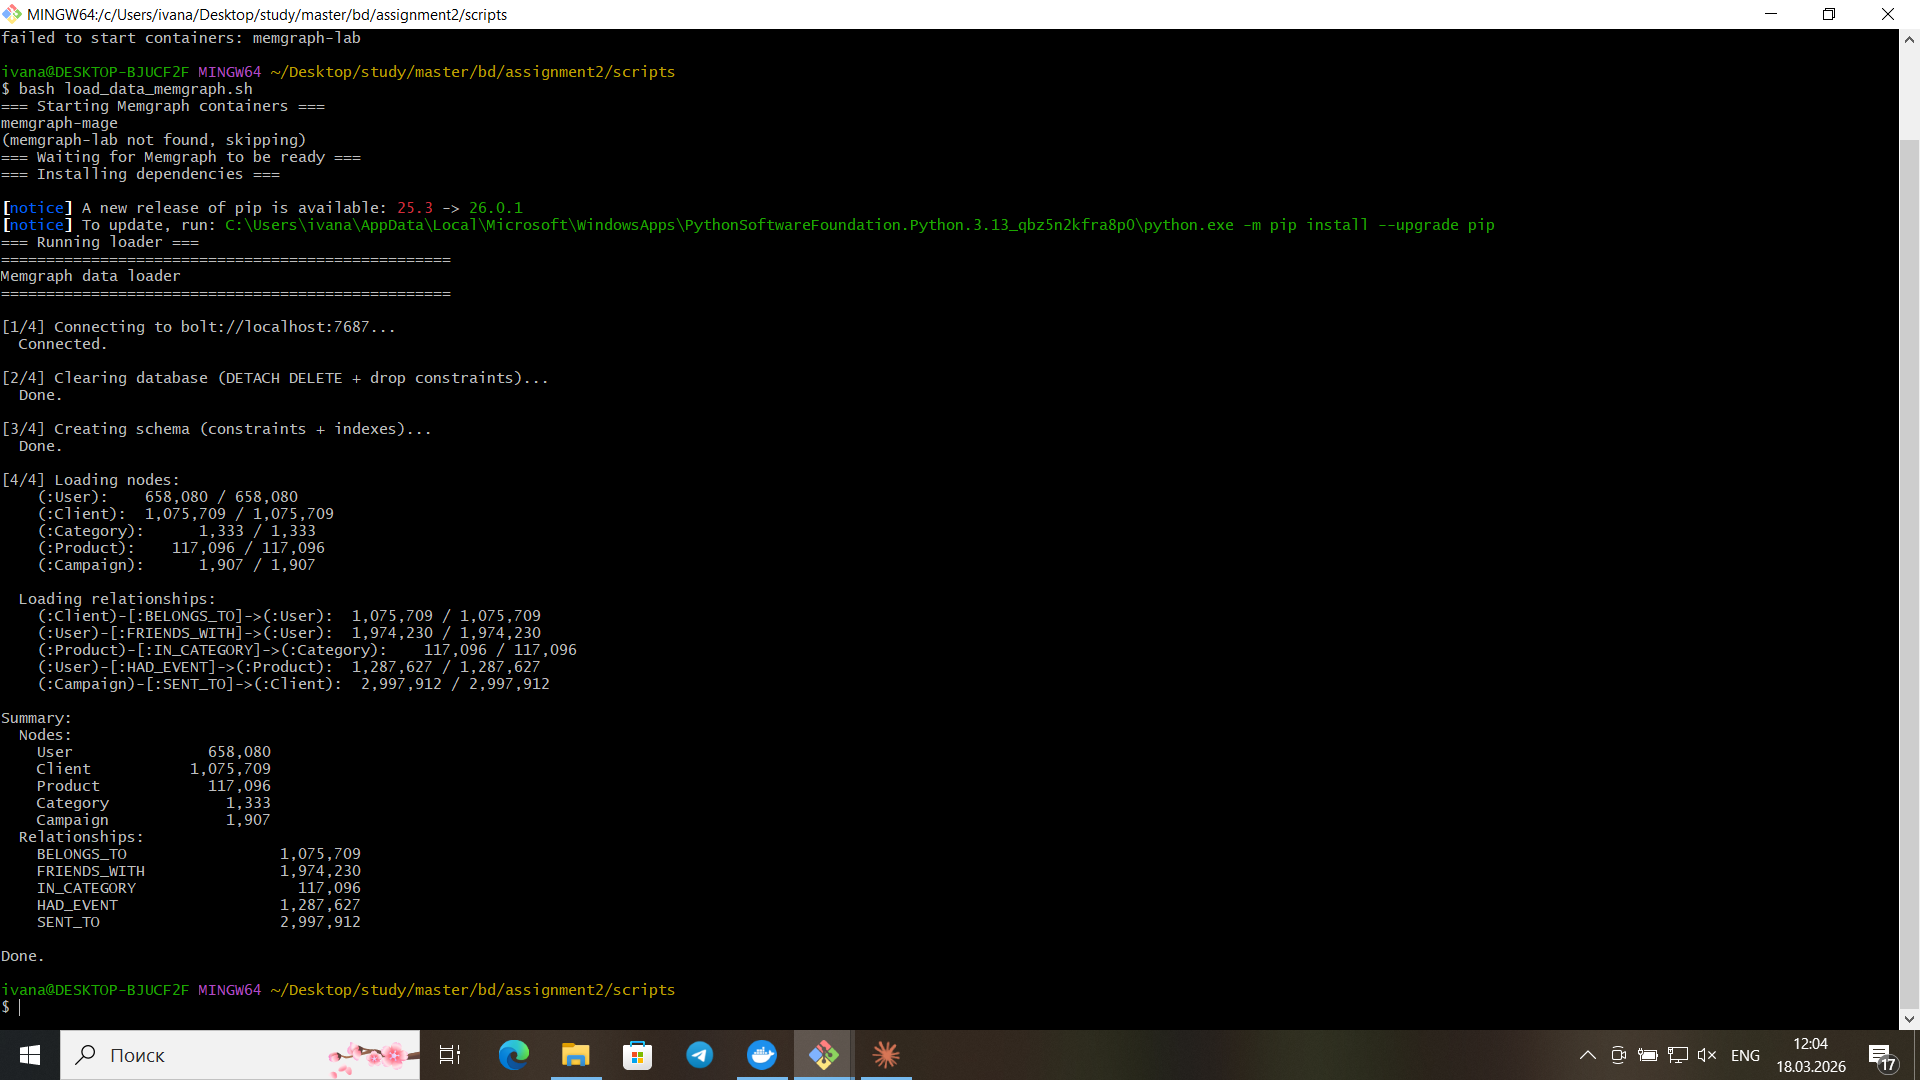
\includegraphics[width=\linewidth]{screenshots/load_data_memgraph.png}
  \caption{Memgraph data loading}
\end{figure}

% ═════════════════════════════════════════════════════════════════════════════
\section{Experimental Results}
% ═════════════════════════════════════════════════════════════════════════════

\subsection{Benchmark Methodology}

Each query script was executed \textbf{6 times} per database: the first run
served as a warm-up (priming OS page cache and database buffer pool) and was
discarded; the subsequent \textbf{5 runs} were recorded. Timing was measured
as wall-clock time from process start to termination, including connection
establishment, query execution, result serialisation, and (where applicable)
pandas post-processing. All results were produced on the same machine with no
other significant workloads running.

\subsection{Query 1a --- Campaign Performance}

\textbf{Semantic goal:} Identify the top-10 marketing campaigns ranked by
purchase conversion rate (purchases / messages sent).

\textbf{Implementation:}
\begin{itemize}
  \item \textbf{PostgreSQL (both models):} \texttt{JOIN messages m ON campaigns c},
        \texttt{GROUP BY campaign\_id}, aggregate boolean flags with
        \texttt{SUM(is\_purchased::int) / COUNT(*)}.
  \item \textbf{MongoDB:} \texttt{\$lookup} messages into campaigns,
        \texttt{\$group} by \texttt{campaign\_id}, compute ratio with
        \texttt{\$divide}.
  \item \textbf{Memgraph:} \texttt{MATCH (msg:Message)-[:PART\_OF]->(c:Campaign)},
        \texttt{WITH c, COUNT/SUM} aggregation, \texttt{ORDER BY} rate.
\end{itemize}

\subsection{Query 1b --- User Targeting Score}

\textbf{Semantic goal:} Score each user for marketing targeting:
$+2$ if the user personally purchased, $+1$ for each friend who purchased.
Return top-20 users.

\textbf{Implementation:}
\begin{itemize}
  \item \textbf{PostgreSQL:} Two CTEs --- \texttt{purchasers} (users who
        bought via messages), \texttt{friend\_score} (union of both
        friendship directions joined to purchasers). Final
        \texttt{SELECT} sums friend score + self-purchase bonus.
  \item \textbf{MongoDB:} \texttt{\$graphLookup} on the
        \texttt{friendships} collection combined with a \texttt{\$lookup}
        on purchased messages. The friend-traversal aggregation proved
        extremely slow ($\approx$1774 s) due to the large number of
        friendship pairs requiring per-document lookups.
  \item \textbf{Memgraph:} Natural fit for graph traversal ---
        \texttt{MATCH (u)-[:FRIENDS\_WITH]-(friend)} pattern with
        purchase flag propagation. Executes in $\approx$2.4 s, far faster
        than MongoDB for this relationship-heavy query.
\end{itemize}

\textbf{Note on MongoDB Q1b performance:} The \texttt{\$lookup} inside an
aggregation pipeline does not benefit from indexes when the join is on a nested
array field. The friendship graph ($N$ users $\times$ average degree) results
in a cross-product scan for each user, making this query fundamentally
ill-suited for a document store.

\begin{figure}[H]
  \centering
  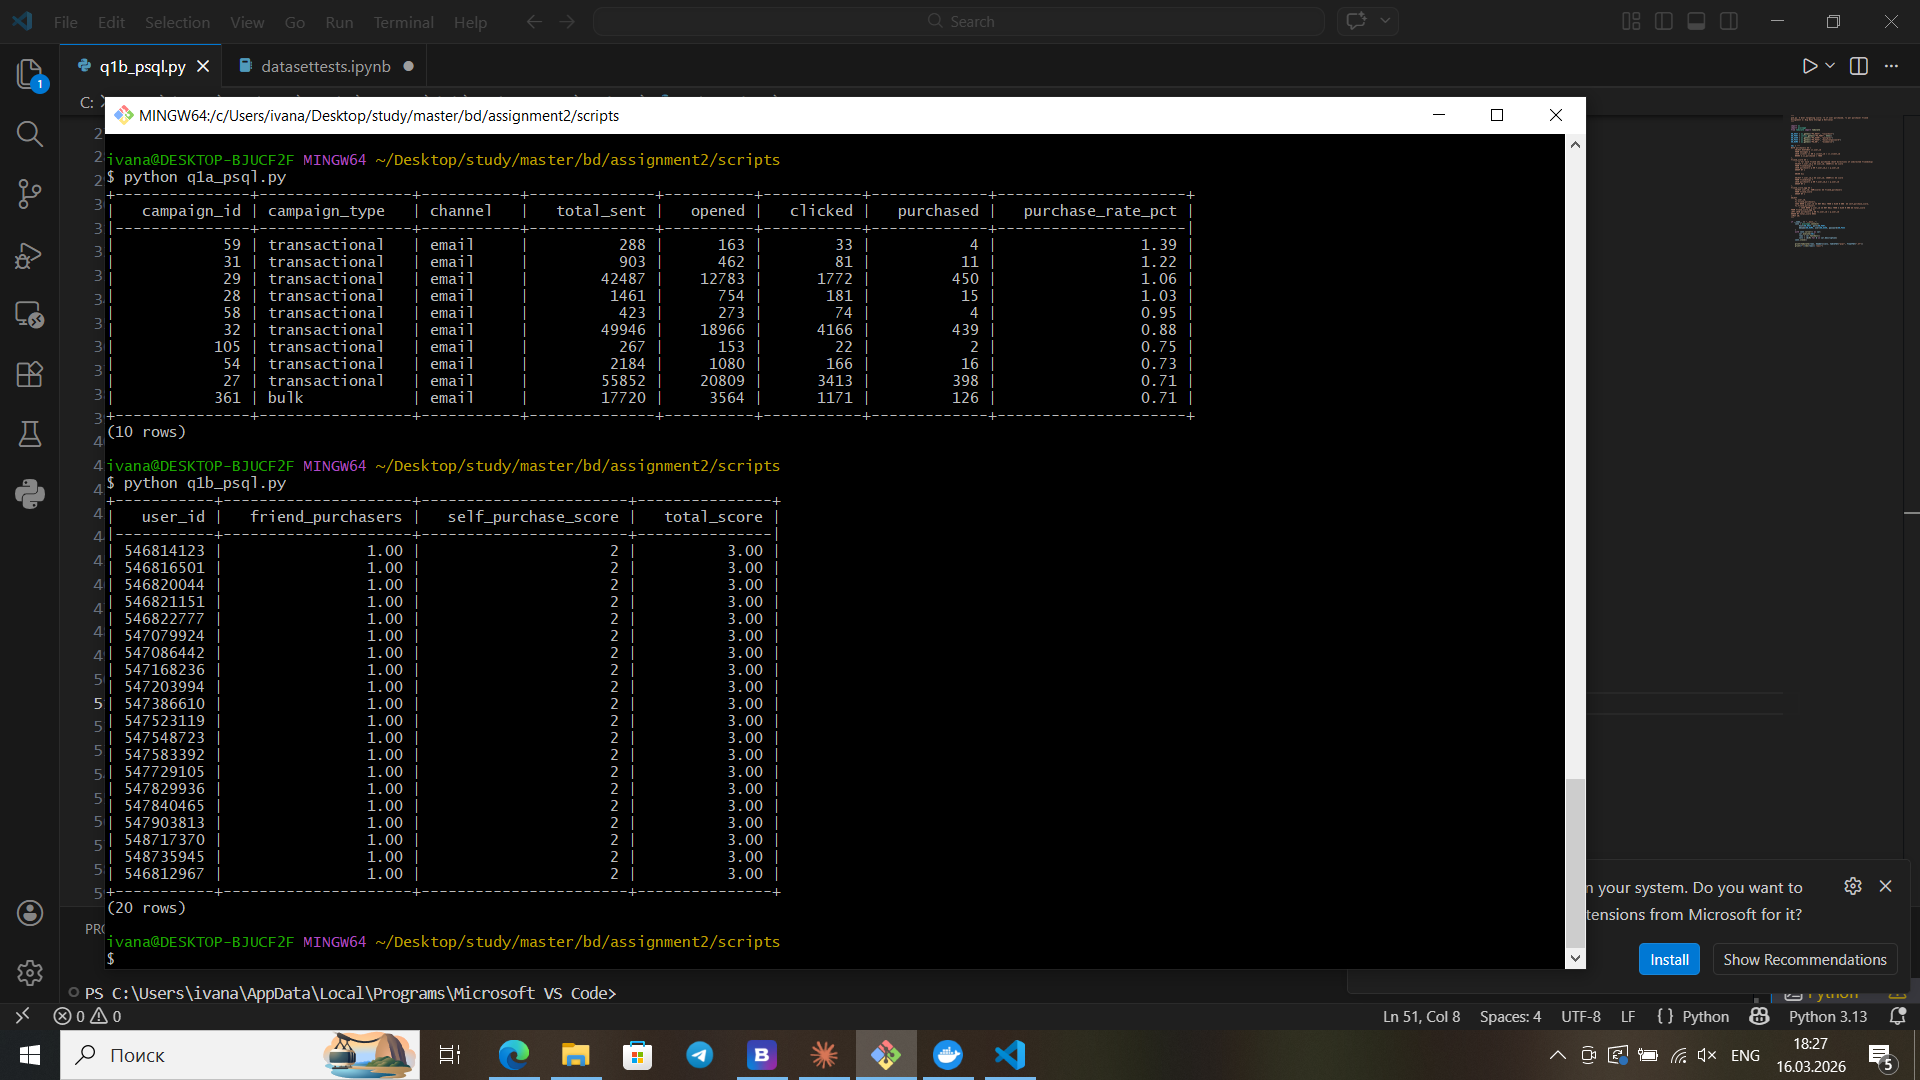
\includegraphics[width=\linewidth]{screenshots/q1_psql.png}
  \caption{Q1 results --- PostgreSQL 3NF}
\end{figure}

\begin{figure}[H]
  \centering
  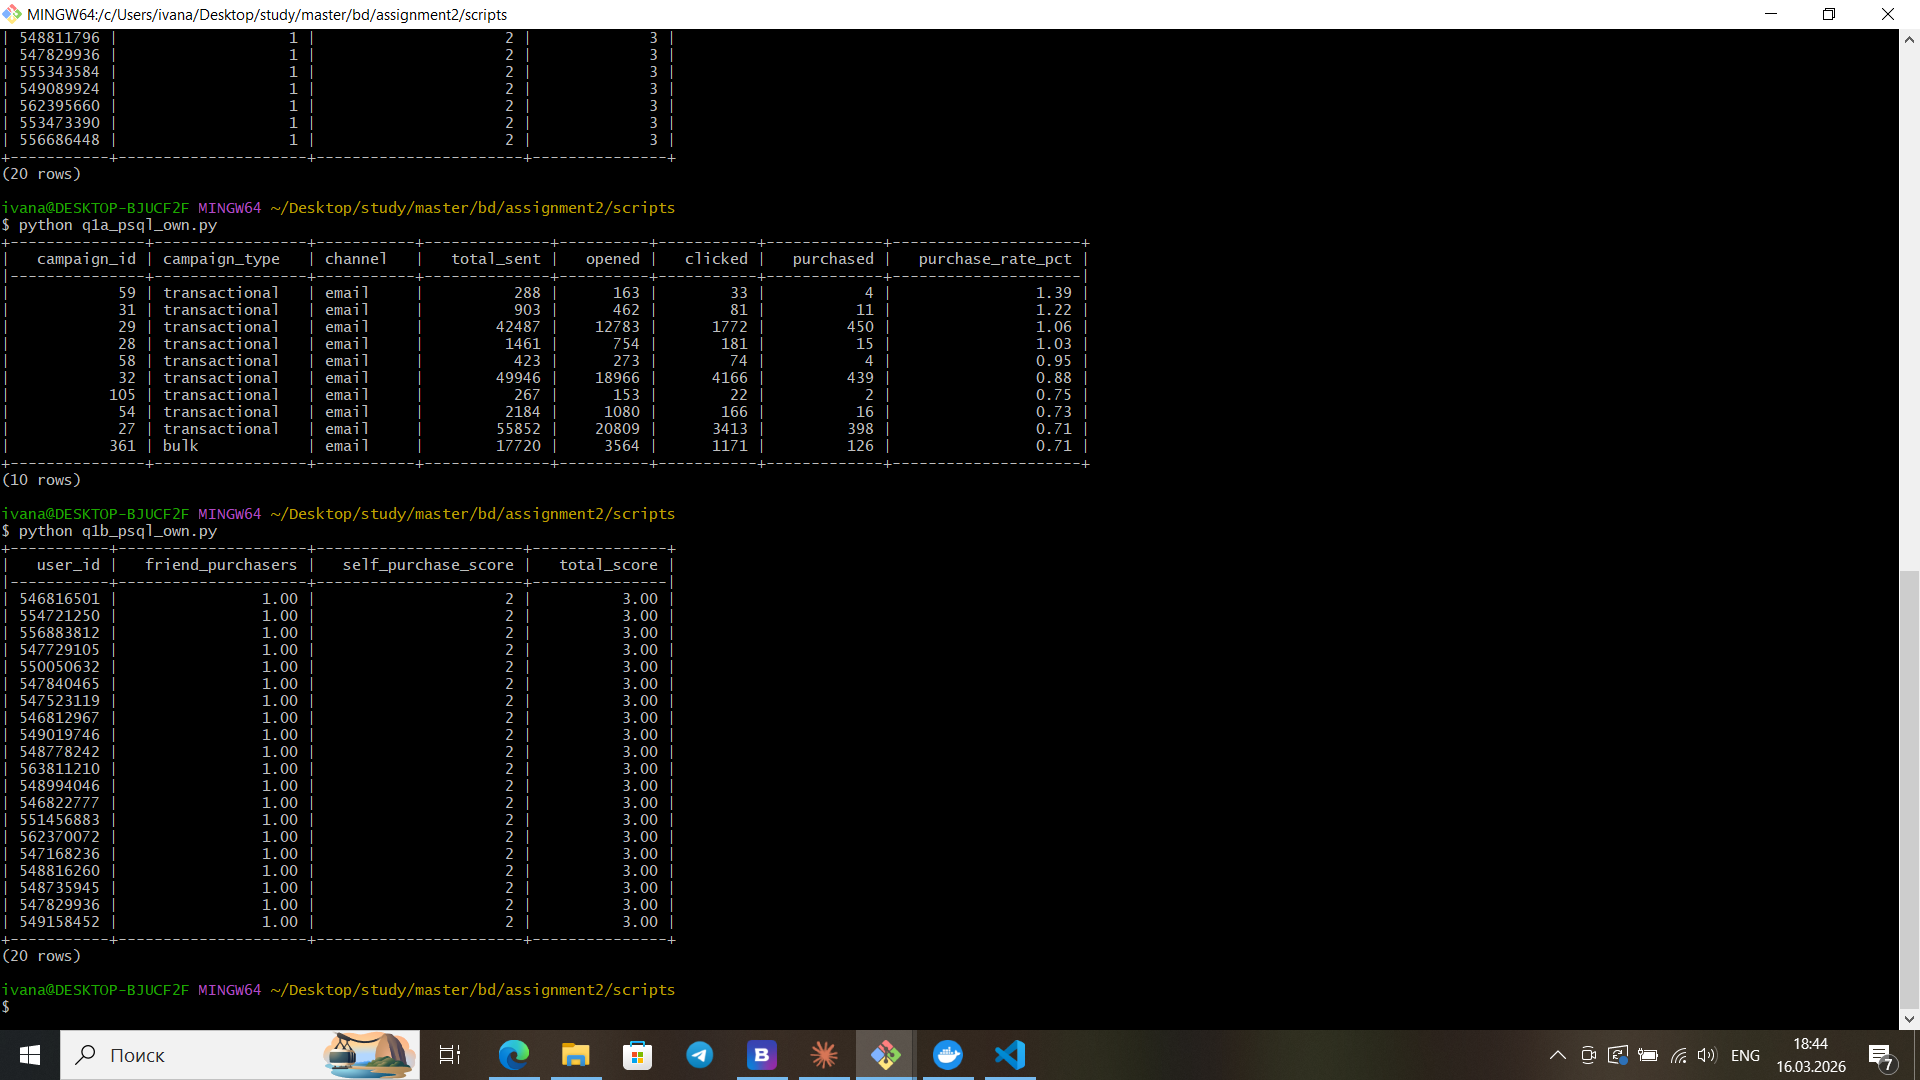
\includegraphics[width=\linewidth]{screenshots/q1_psql_own.png}
  \caption{Q1 results --- PostgreSQL Own}
\end{figure}

\begin{figure}[H]
  \centering
  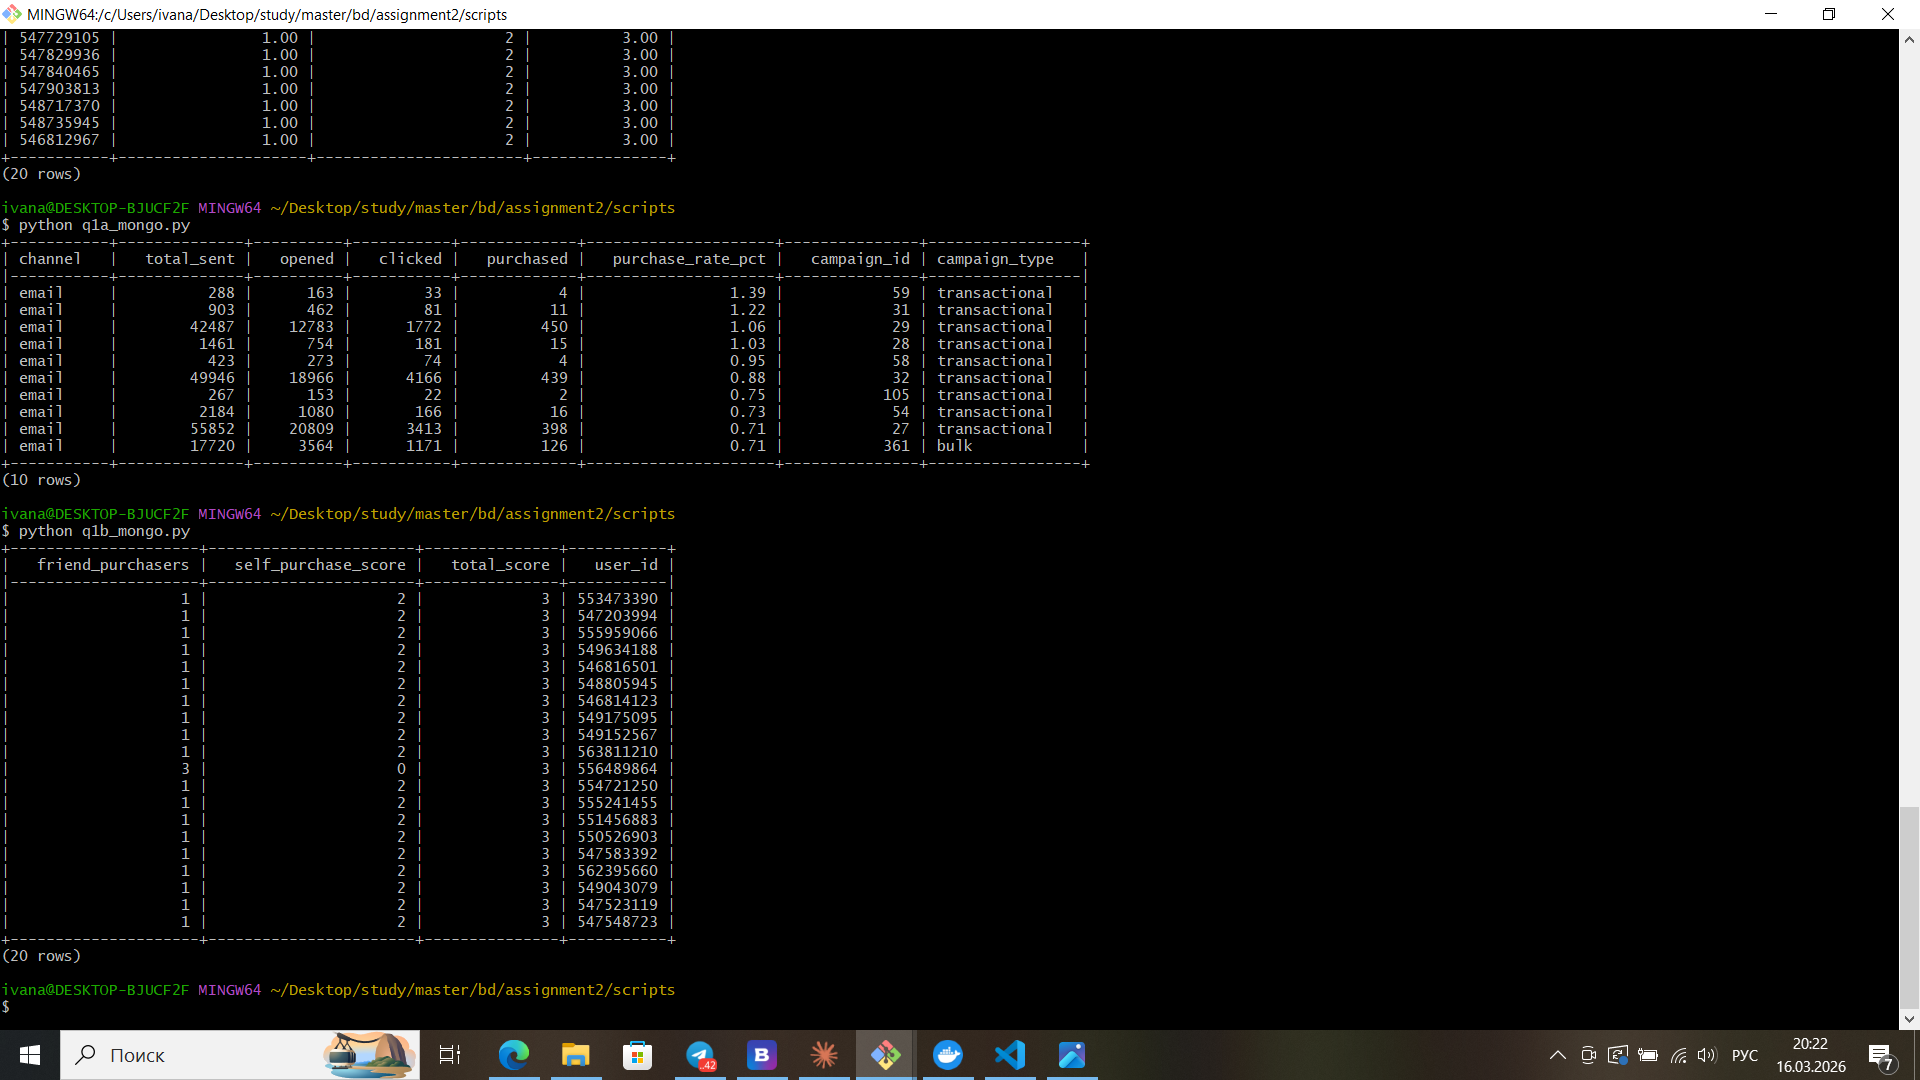
\includegraphics[width=\linewidth]{screenshots/q1_mongo.png}
  \caption{Q1 results --- MongoDB}
\end{figure}

\begin{figure}[H]
  \centering
  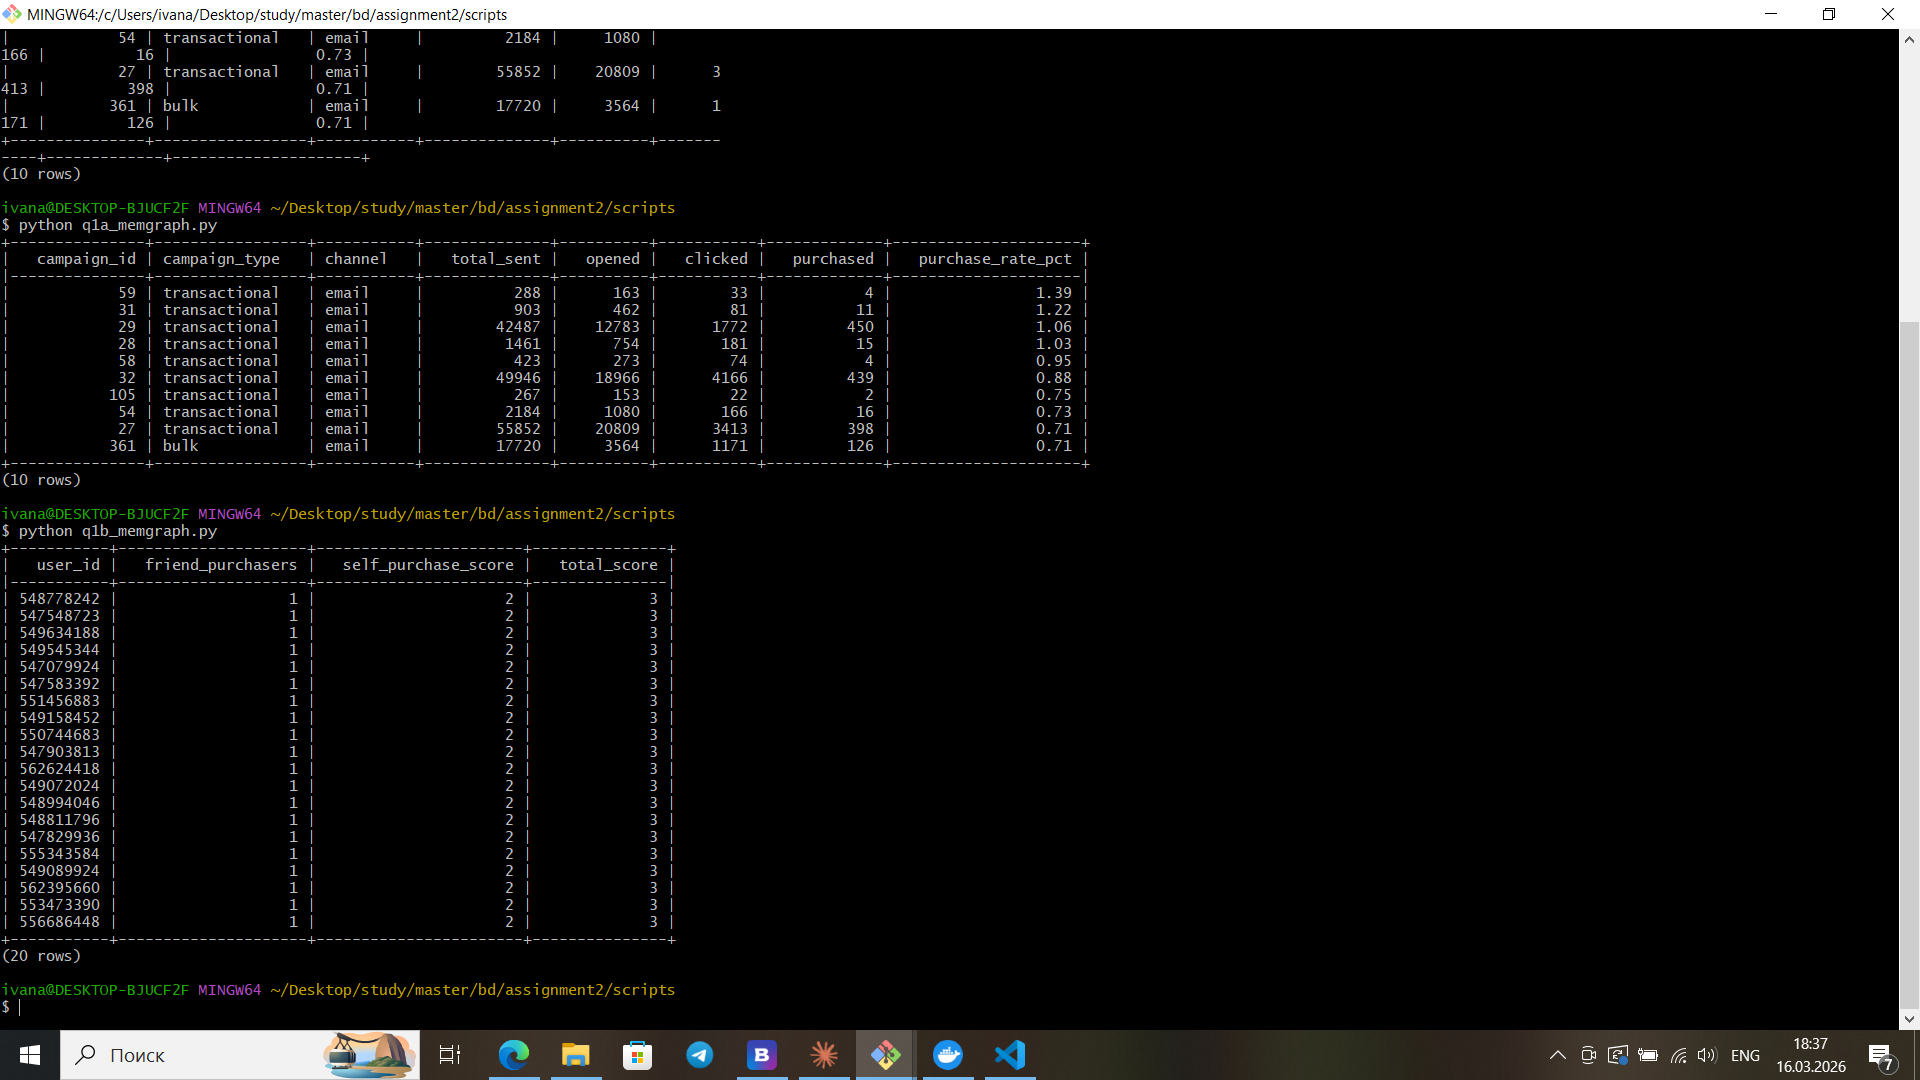
\includegraphics[width=\linewidth]{screenshots/q1_memgraph.png}
  \caption{Q1 results --- Memgraph}
\end{figure}

\subsection{Query 2 --- Personalised Product Recommendations}

\textbf{Semantic goal:} For each user, score categories by weighted interaction
history (purchase=3, cart=2, view=1), select the top-3 preferred categories,
then recommend the top-5 most globally-purchased products per category that the
user has not yet bought.

\textbf{Implementation:}
\begin{itemize}
  \item \textbf{PostgreSQL (both models):} A chain of CTEs:
        \texttt{event\_scores} $\to$ \texttt{category\_scores} $\to$
        \texttt{top\_categories} (with \texttt{ROW\_NUMBER}) $\to$
        \texttt{product\_popularity} $\to$ \texttt{top\_products}
        (\texttt{PARTITION BY category\_sk}) $\to$
        \texttt{already\_purchased} (excluded by \texttt{product\_sk}).
        The \emph{Own} model is $\approx40\%$ faster because category
        attributes are inline in \texttt{events}, avoiding a join to
        \texttt{products}.
  \item \textbf{MongoDB:} The initial single-pipeline implementation used
        a \emph{correlated} \texttt{\$lookup} on the \texttt{events}
        collection for every (user, category) pair, resulting in
        $O(N_\text{users} \times N_\text{cats} \times N_\text{events})$
        complexity and a runtime of $\approx$5500 s. This was redesigned
        as \textbf{four independent aggregation pipelines} followed by
        pandas merges, reducing runtime to $\approx$1773 s. The dominant
        cost is the \texttt{PIPELINE\_CAT\_SCORES} step which performs a
        \texttt{\$lookup} of all events to products.
  \item \textbf{Memgraph:} A single Cypher query computing global purchase
        counts per product timed out after 8+ hours. The query was split
        into \textbf{four separate Cypher queries} (category scores,
        global popularity, product-category mapping, purchased set) with
        pandas aggregation, converging to $\approx$396 s. The bottleneck
        is the \texttt{COUNT} of all \texttt{HAD\_EVENT} relationships per
        product node.
\end{itemize}

\begin{figure}[H]
  \centering
  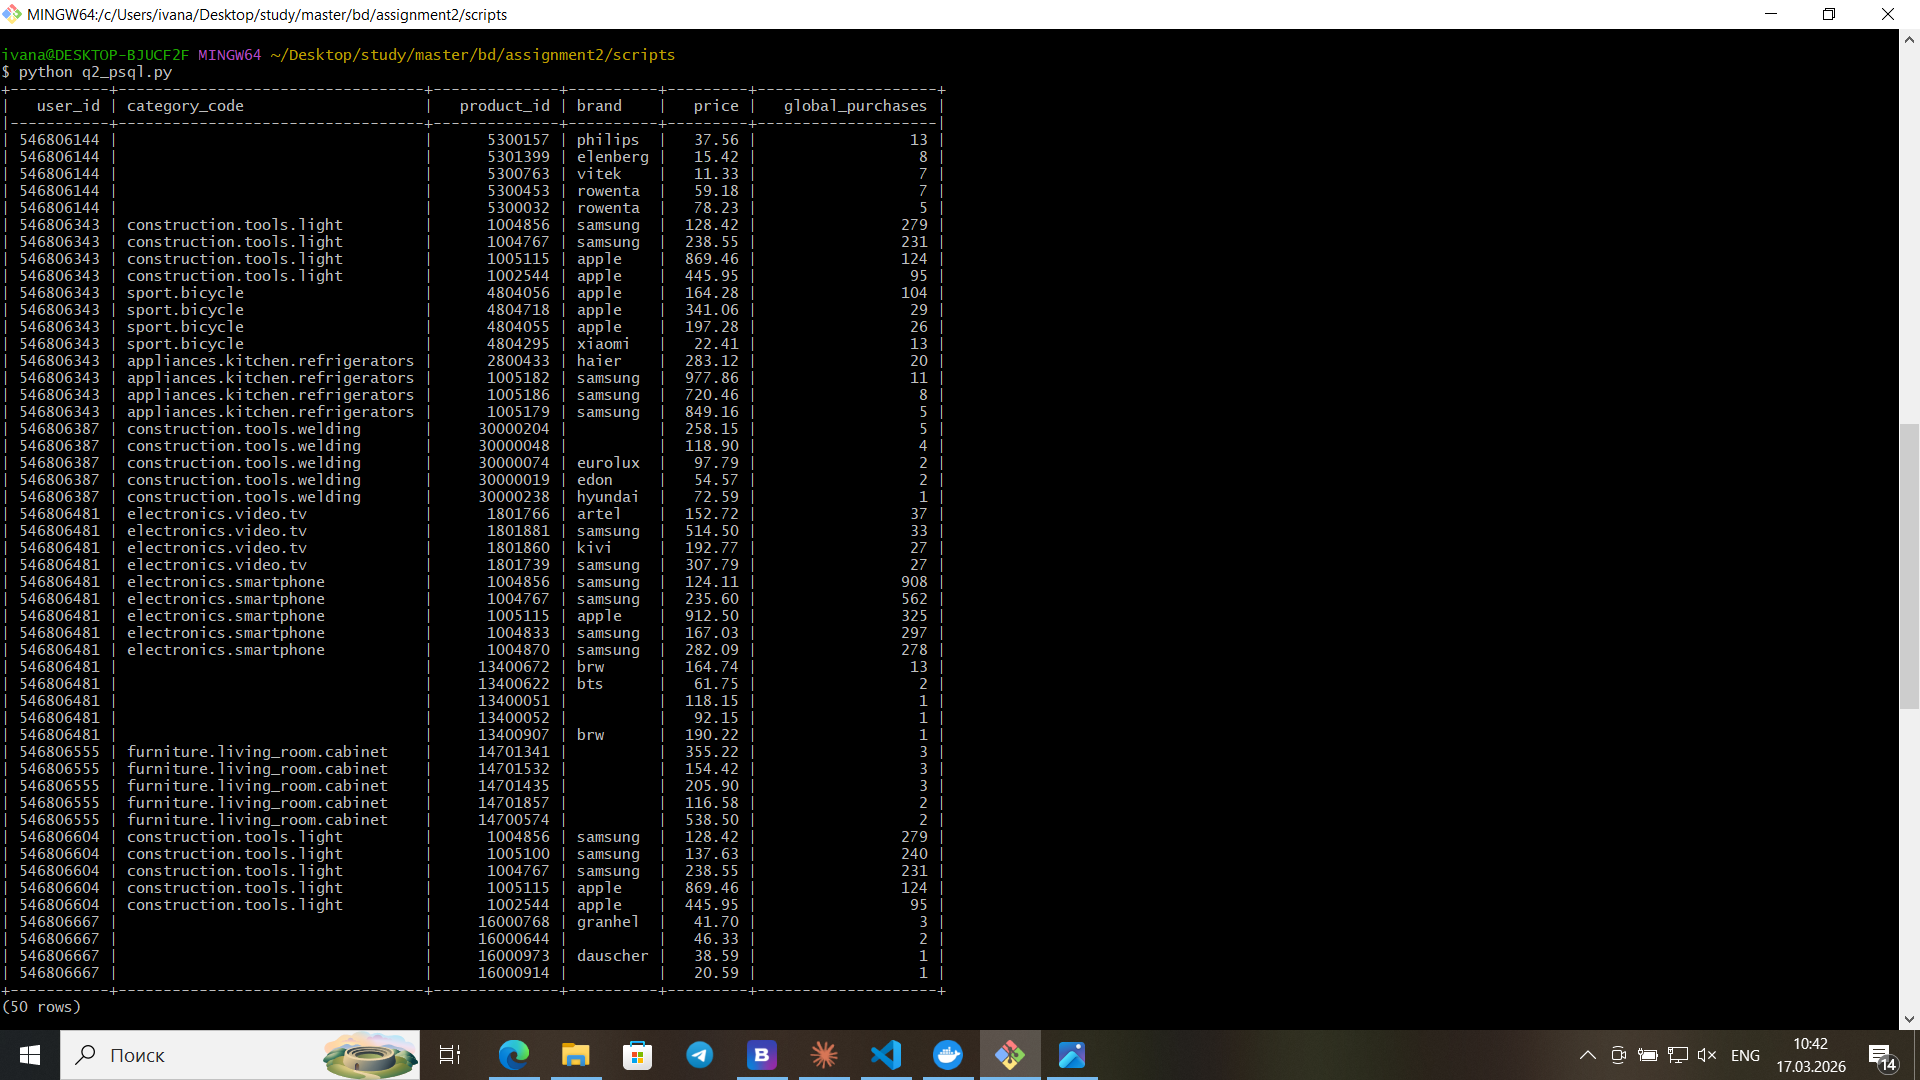
\includegraphics[width=\linewidth]{screenshots/q2_psql.png}
  \caption{Q2 results --- PostgreSQL 3NF}
\end{figure}

\begin{figure}[H]
  \centering
  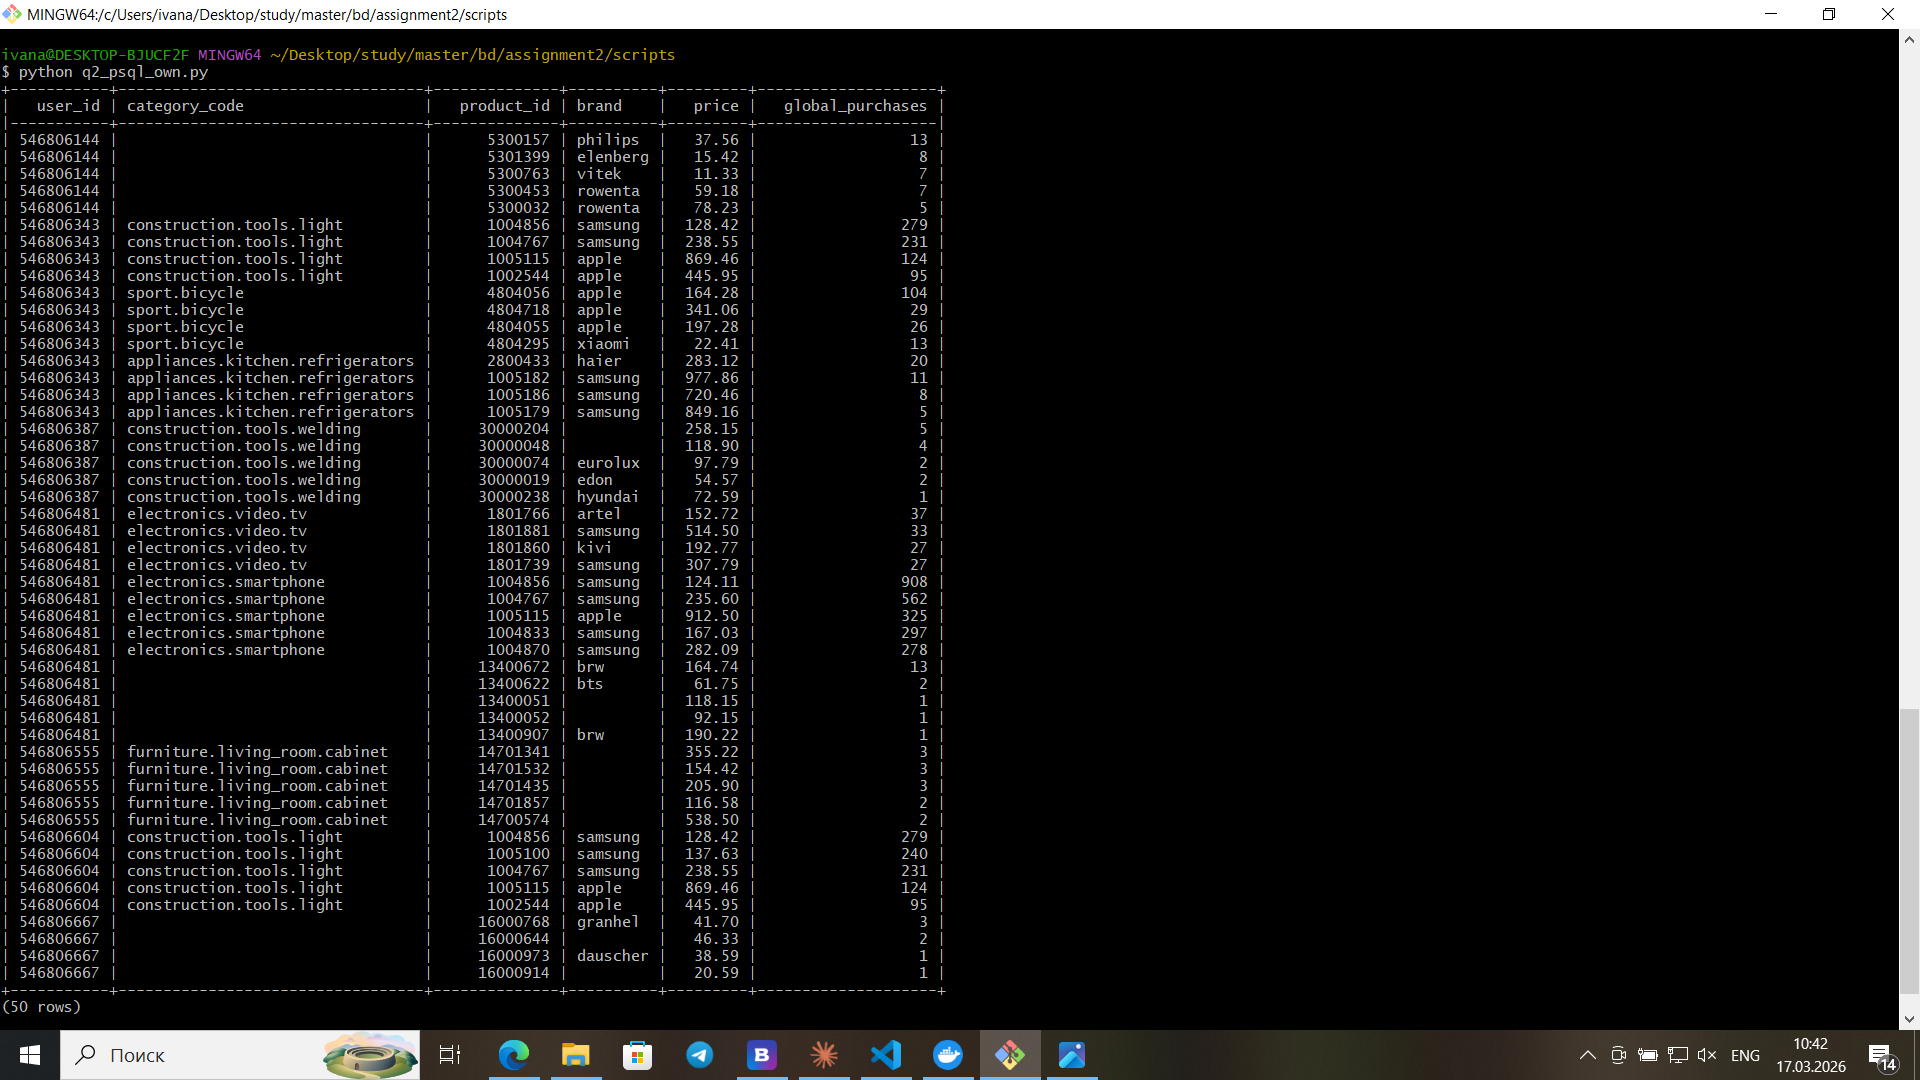
\includegraphics[width=\linewidth]{screenshots/q2_psql_own.png}
  \caption{Q2 results --- PostgreSQL Own}
\end{figure}

\begin{figure}[H]
  \centering
  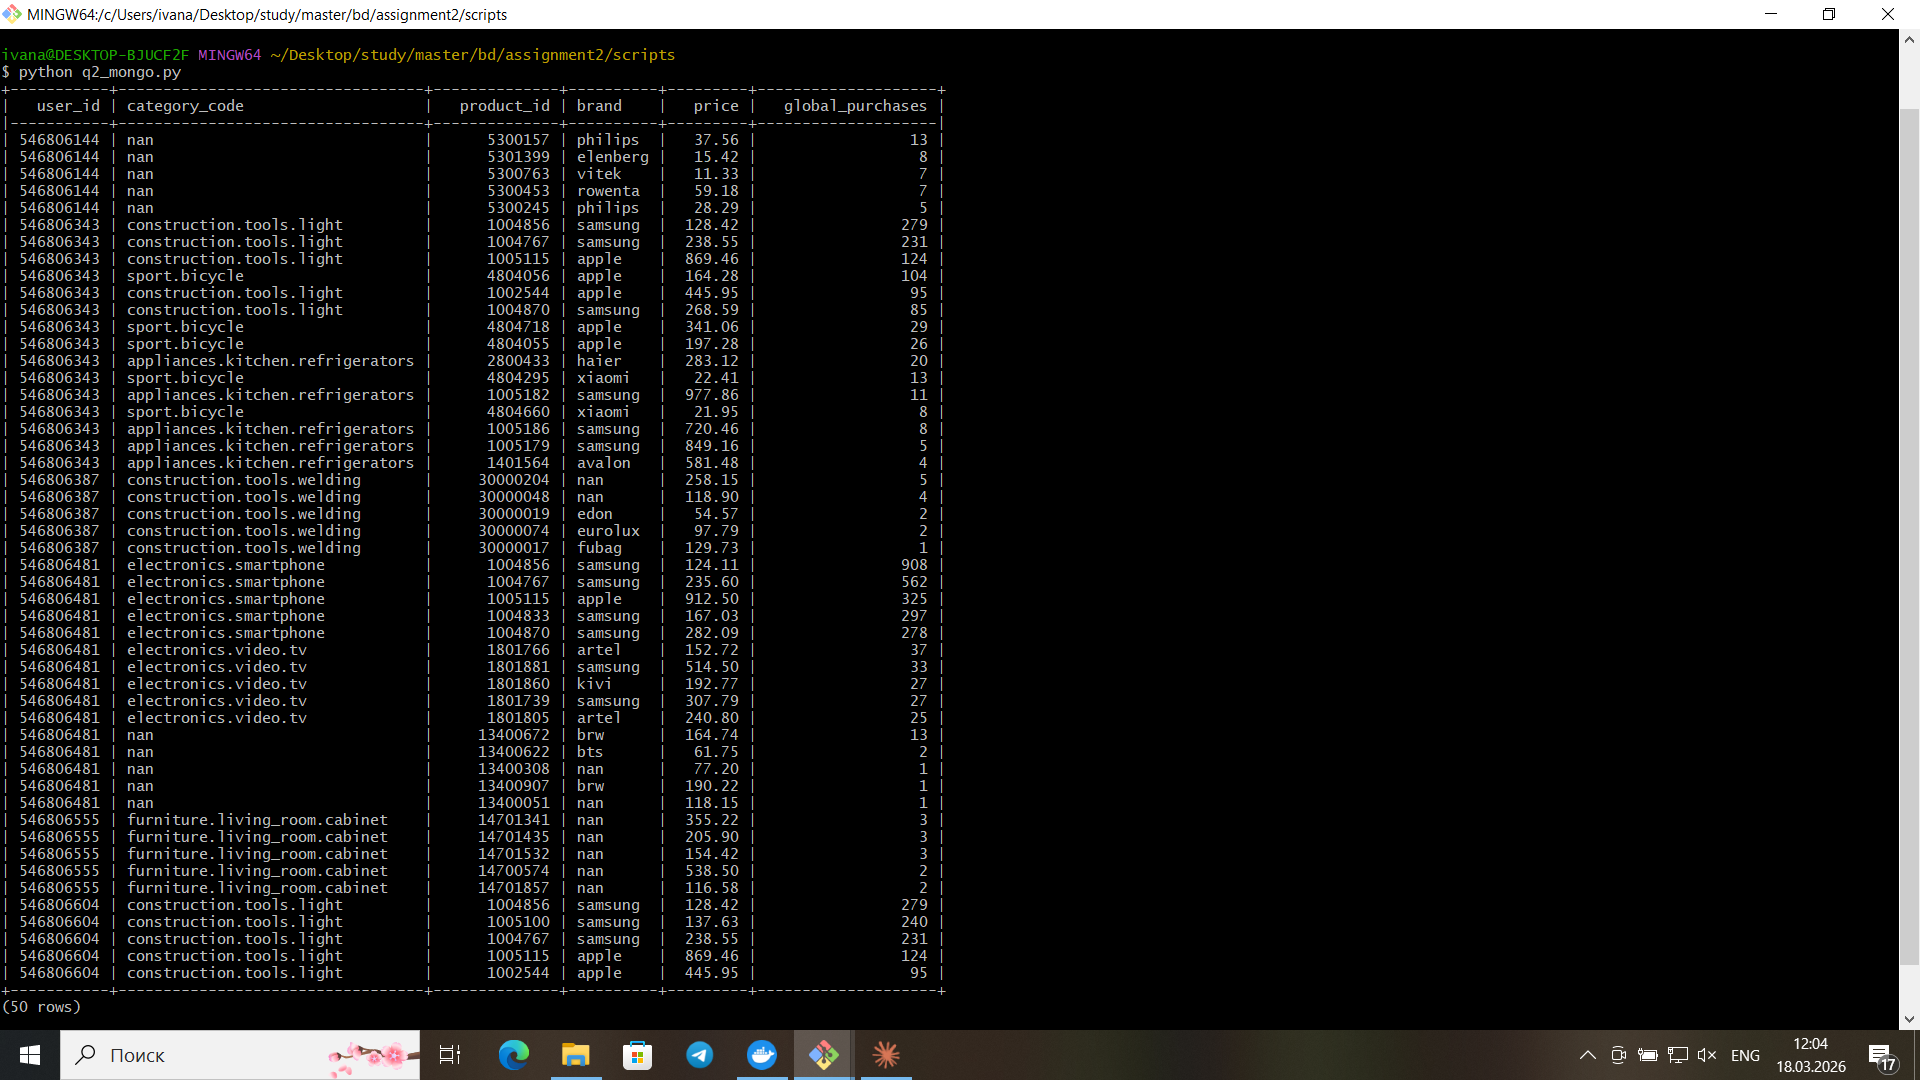
\includegraphics[width=\linewidth]{screenshots/q2_mongo.png}
  \caption{Q2 results --- MongoDB}
\end{figure}

\begin{figure}[H]
  \centering
  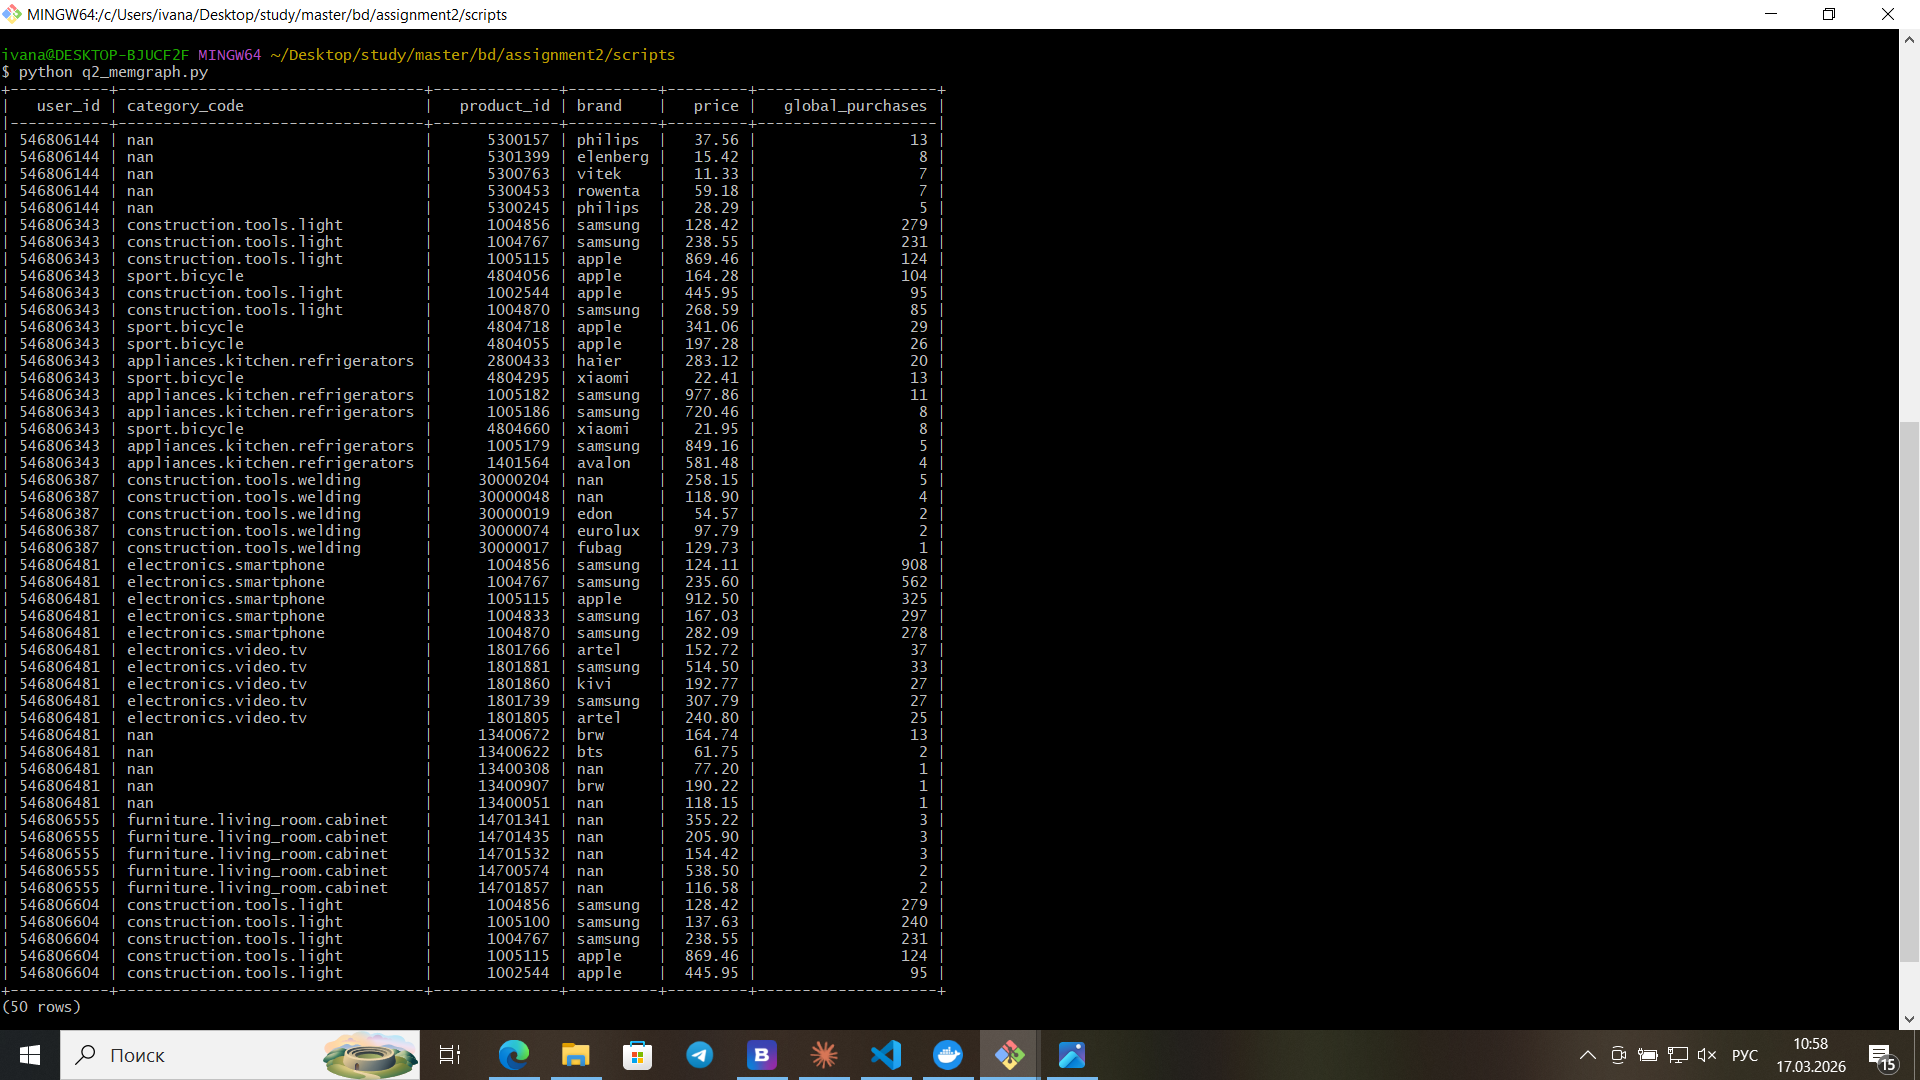
\includegraphics[width=\linewidth]{screenshots/q2_memgraph.png}
  \caption{Q2 results --- Memgraph}
\end{figure}

\subsection{Query 3 --- Full-Text Product Search}

\textbf{Semantic goal:} Given keywords derived from the last segment of
top category codes (``light'', ``bicycle'', ``refrigerators'', ``tv''),
find the top-5 most globally purchased products in each matching category.

\textbf{Implementation:}
\begin{itemize}
  \item \textbf{PostgreSQL:} \texttt{to\_tsvector('simple', REPLACE(category\_code,
        '.', ' ')) @@ to\_tsquery('simple', keyword)} matches categories
        whose dot-separated code contains the keyword as a token.
        Products are ranked by \texttt{buy\_count} from a \texttt{global\_pop}
        CTE; top-5 selected per keyword via \texttt{ROW\_NUMBER() OVER
        (PARTITION BY keyword)}.
  \item \textbf{MongoDB:} \texttt{\$regexMatch} on
        \texttt{category\_code} to find matching categories, followed by a
        \texttt{\$lookup} to events for global purchase counts.
  \item \textbf{Memgraph:} Since Memgraph has no native \texttt{tsvector},
        the Cypher predicate \texttt{cat.category\_code CONTAINS keyword}
        is used as a substring match. Global purchase count is computed
        inline as \texttt{SIZE([()-[:HAD\_EVENT \{event\_type:'purchase'\}]
        ->(p) | 1])}. This list-comprehension count proved very slow
        ($\approx$1215 s) because it traverses all purchase edges for
        every candidate product node.
\end{itemize}

Products within each matching category are ranked by \texttt{global\_purchases}
(total purchase event count across all users), returning the five most
popular items per keyword.

\begin{figure}[H]
  \centering
  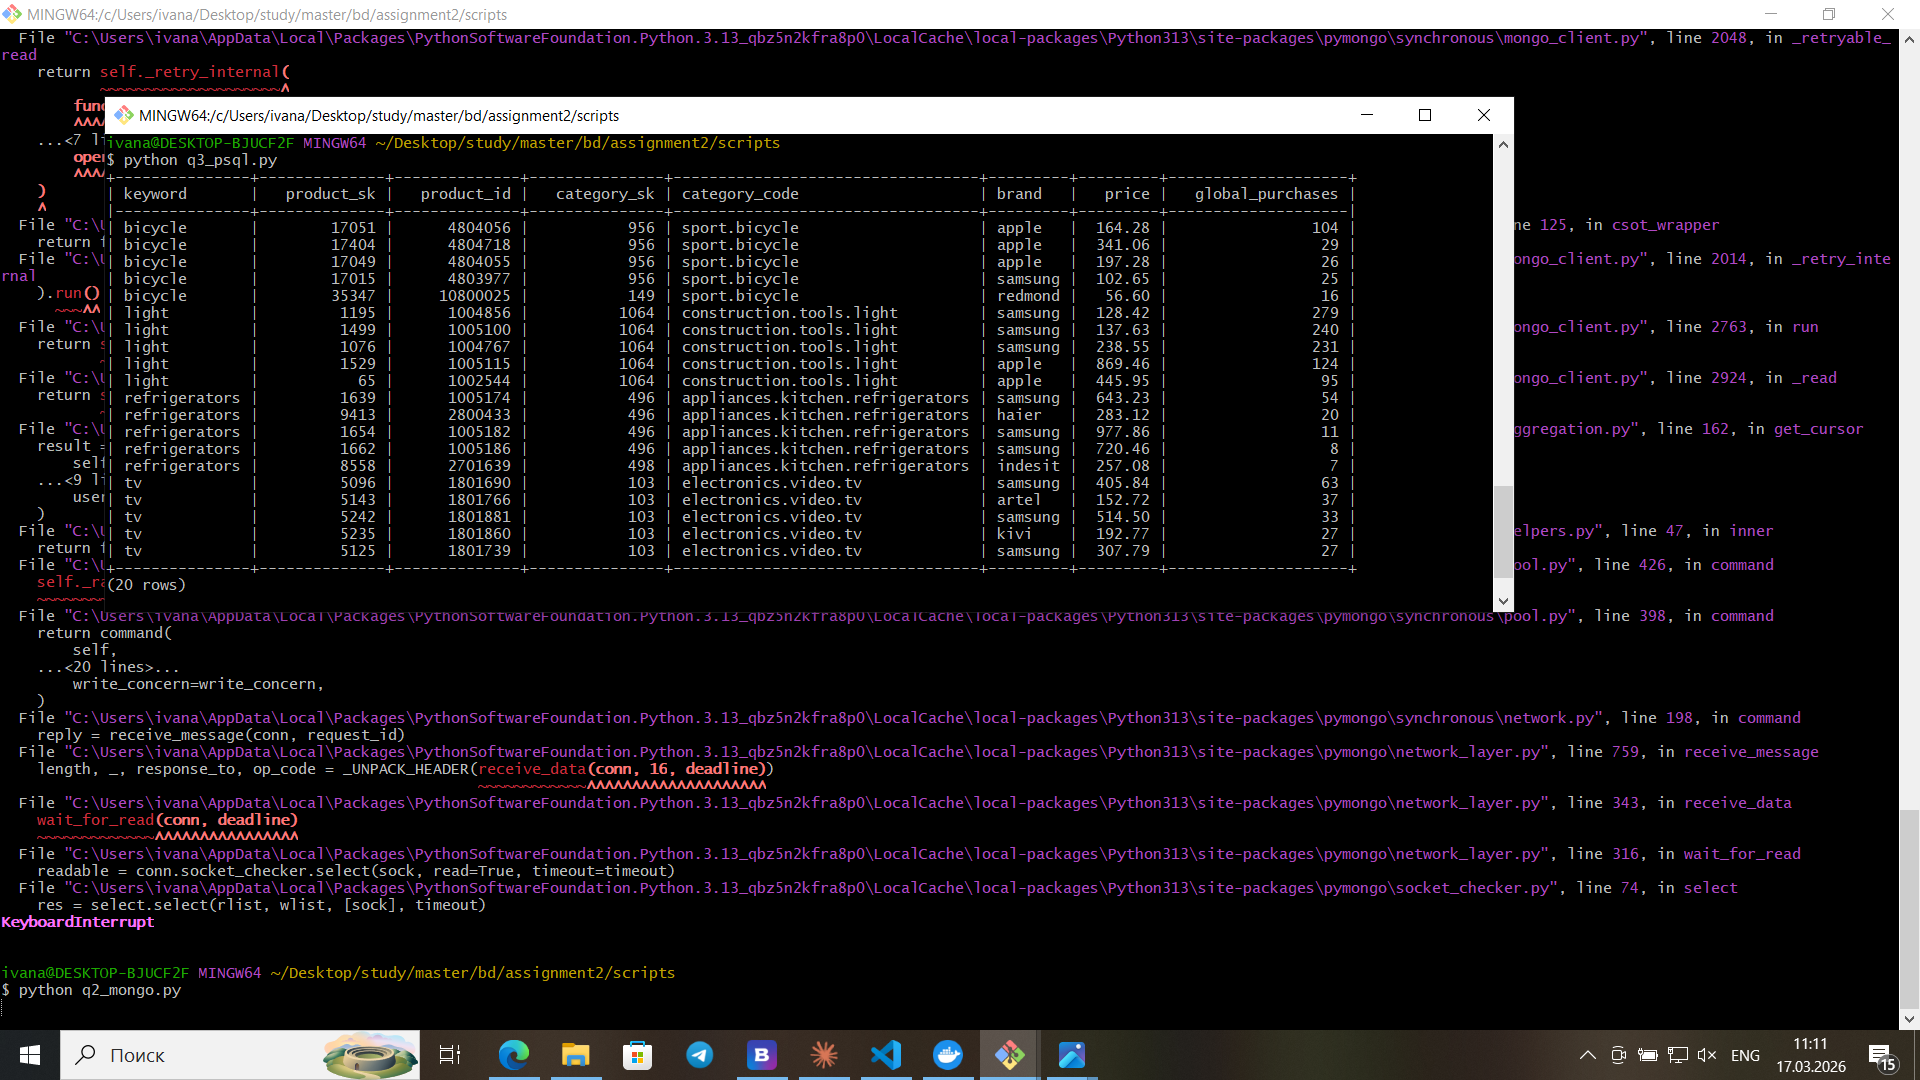
\includegraphics[width=\linewidth]{screenshots/q3_psql.png}
  \caption{Q3 results --- PostgreSQL 3NF}
\end{figure}

\begin{figure}[H]
  \centering
  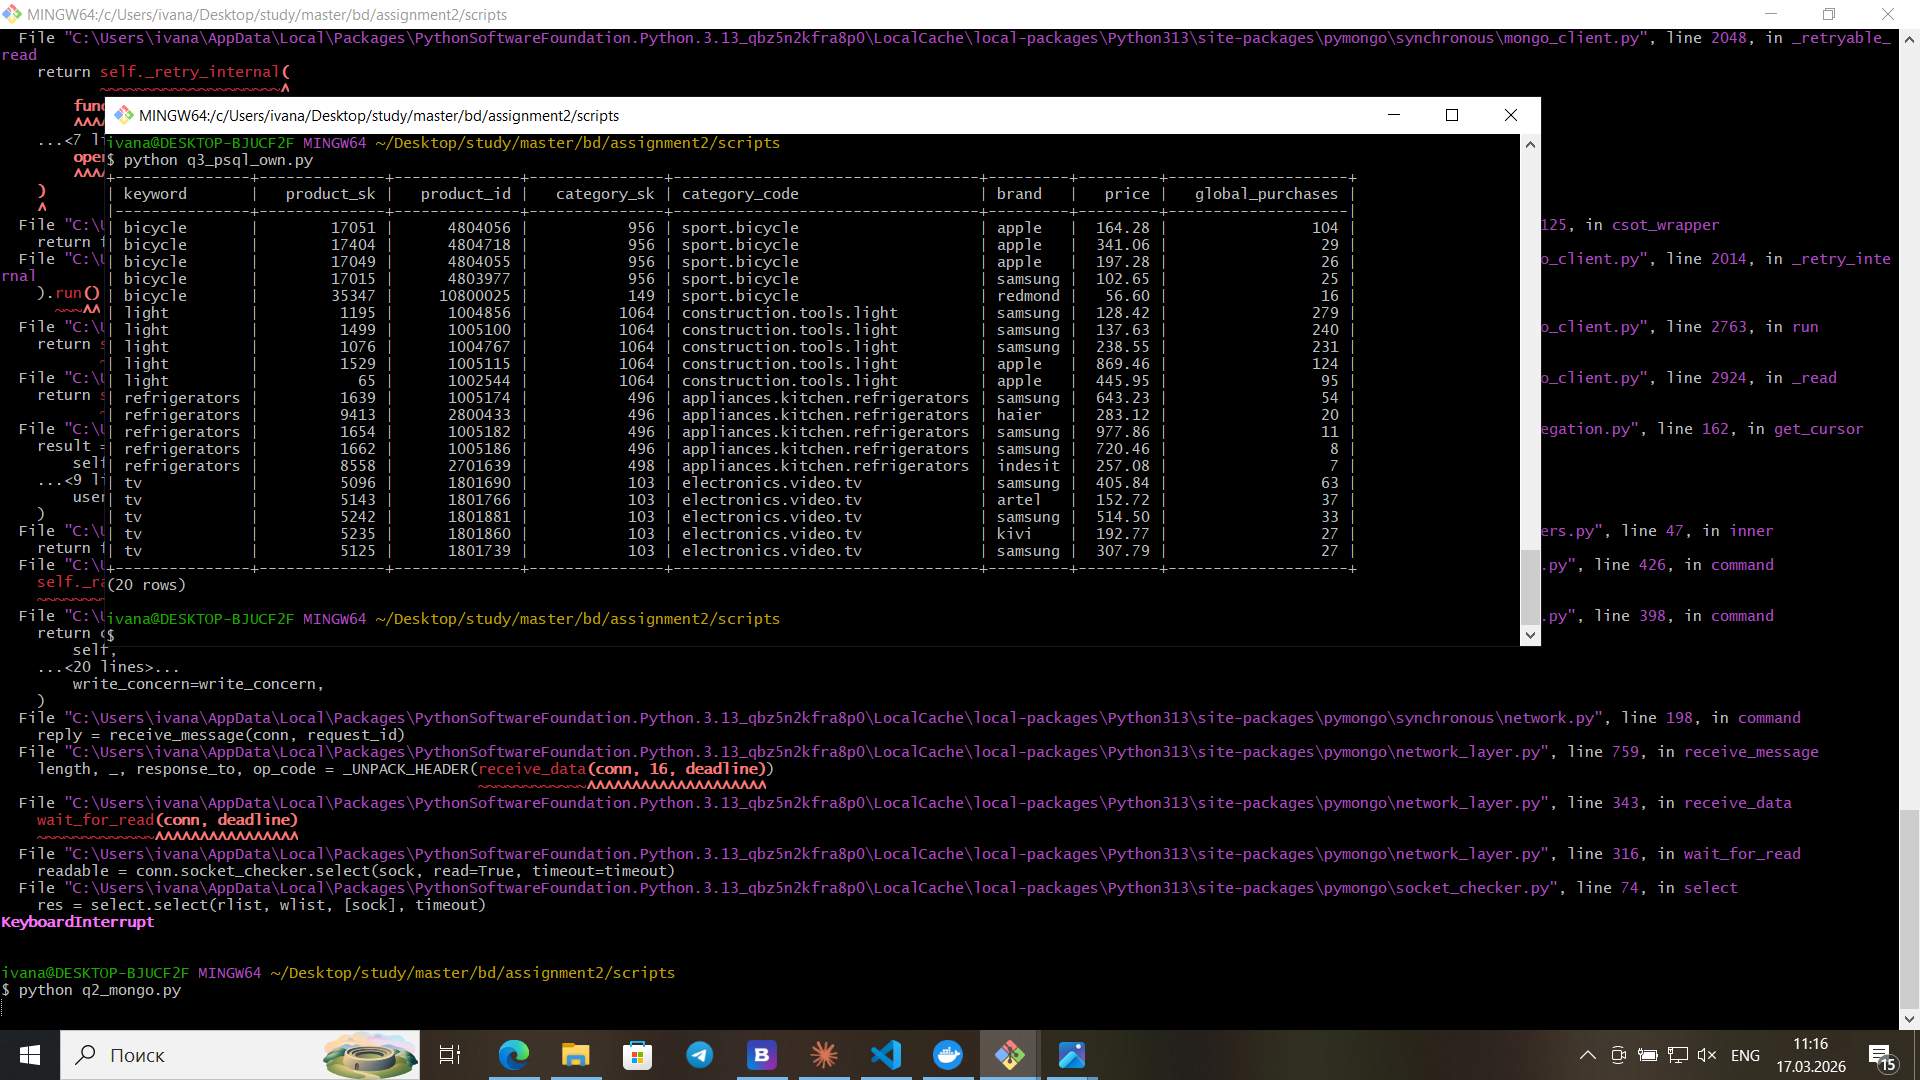
\includegraphics[width=\linewidth]{screenshots/q3_psql_own.png}
  \caption{Q3 results --- PostgreSQL Own}
\end{figure}

\begin{figure}[H]
  \centering
  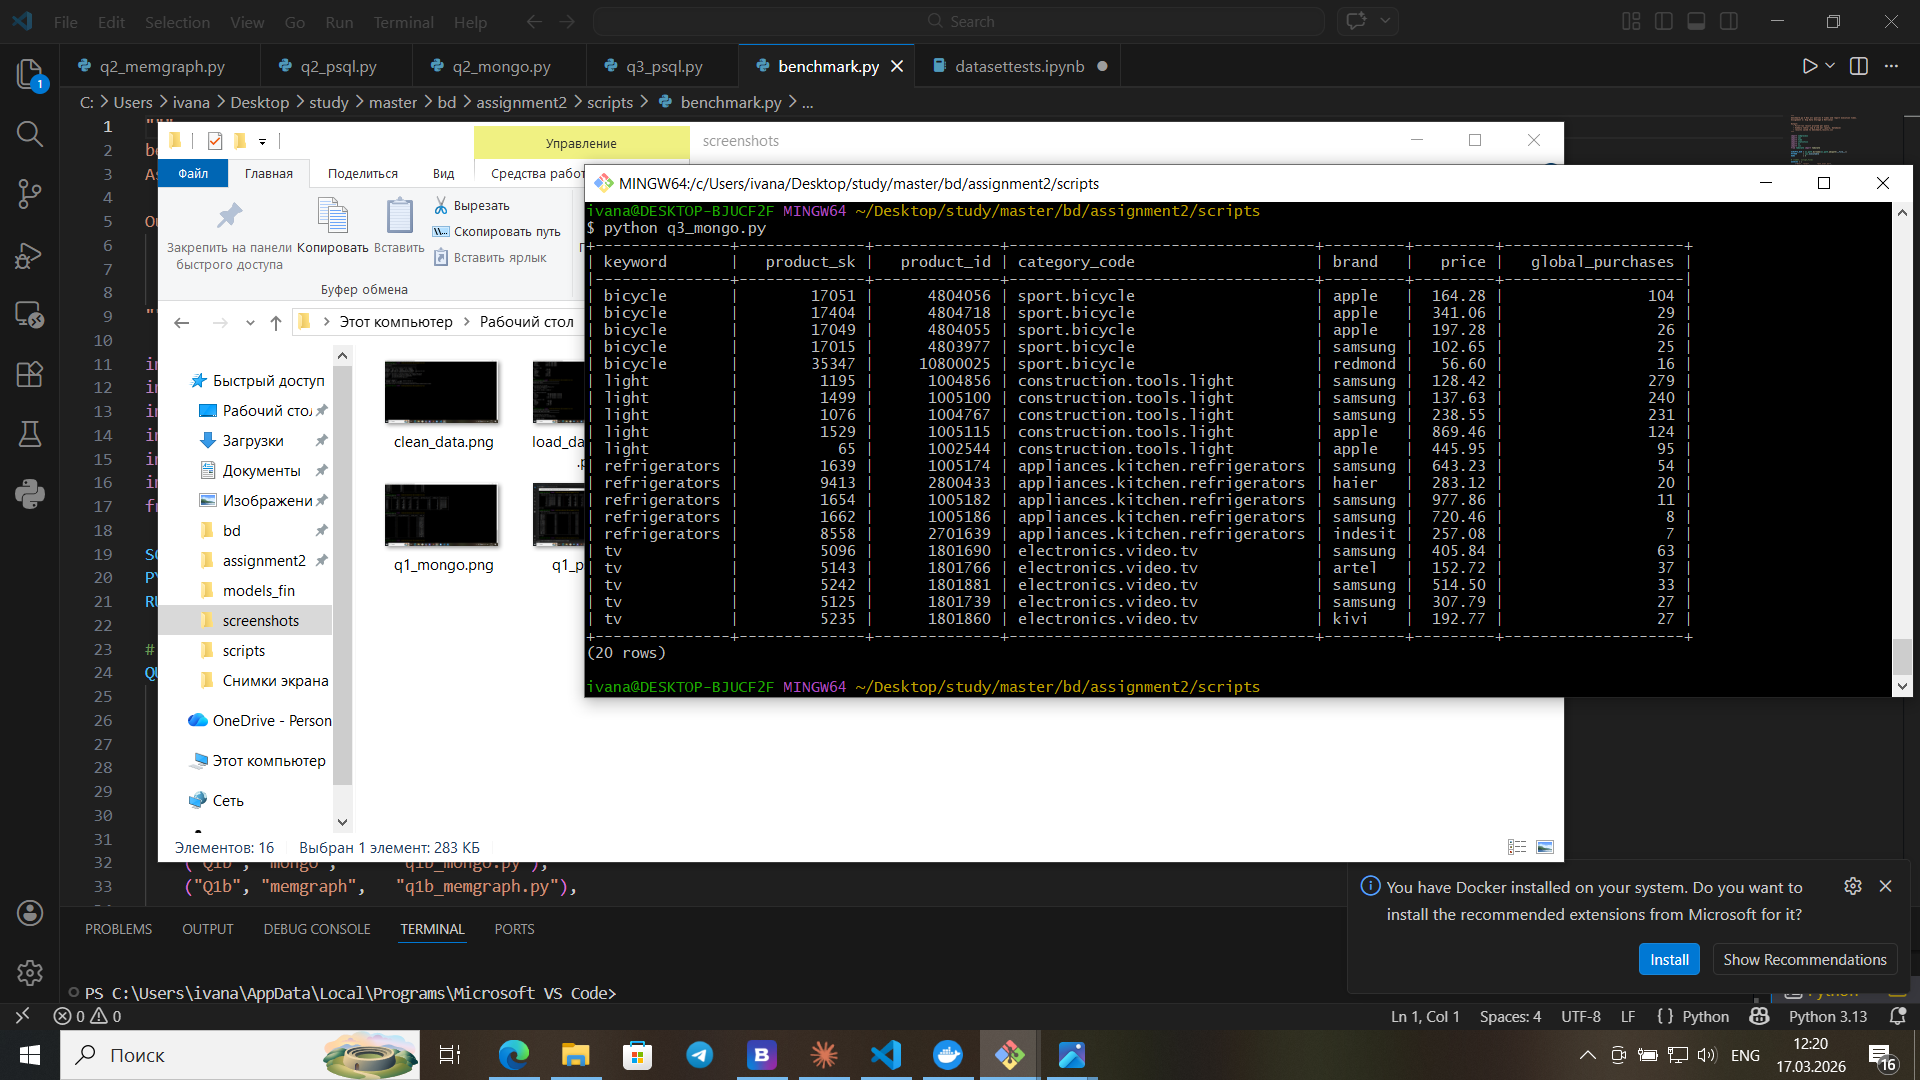
\includegraphics[width=\linewidth]{screenshots/q3_mongo.png}
  \caption{Q3 results --- MongoDB}
\end{figure}

\begin{figure}[H]
  \centering
  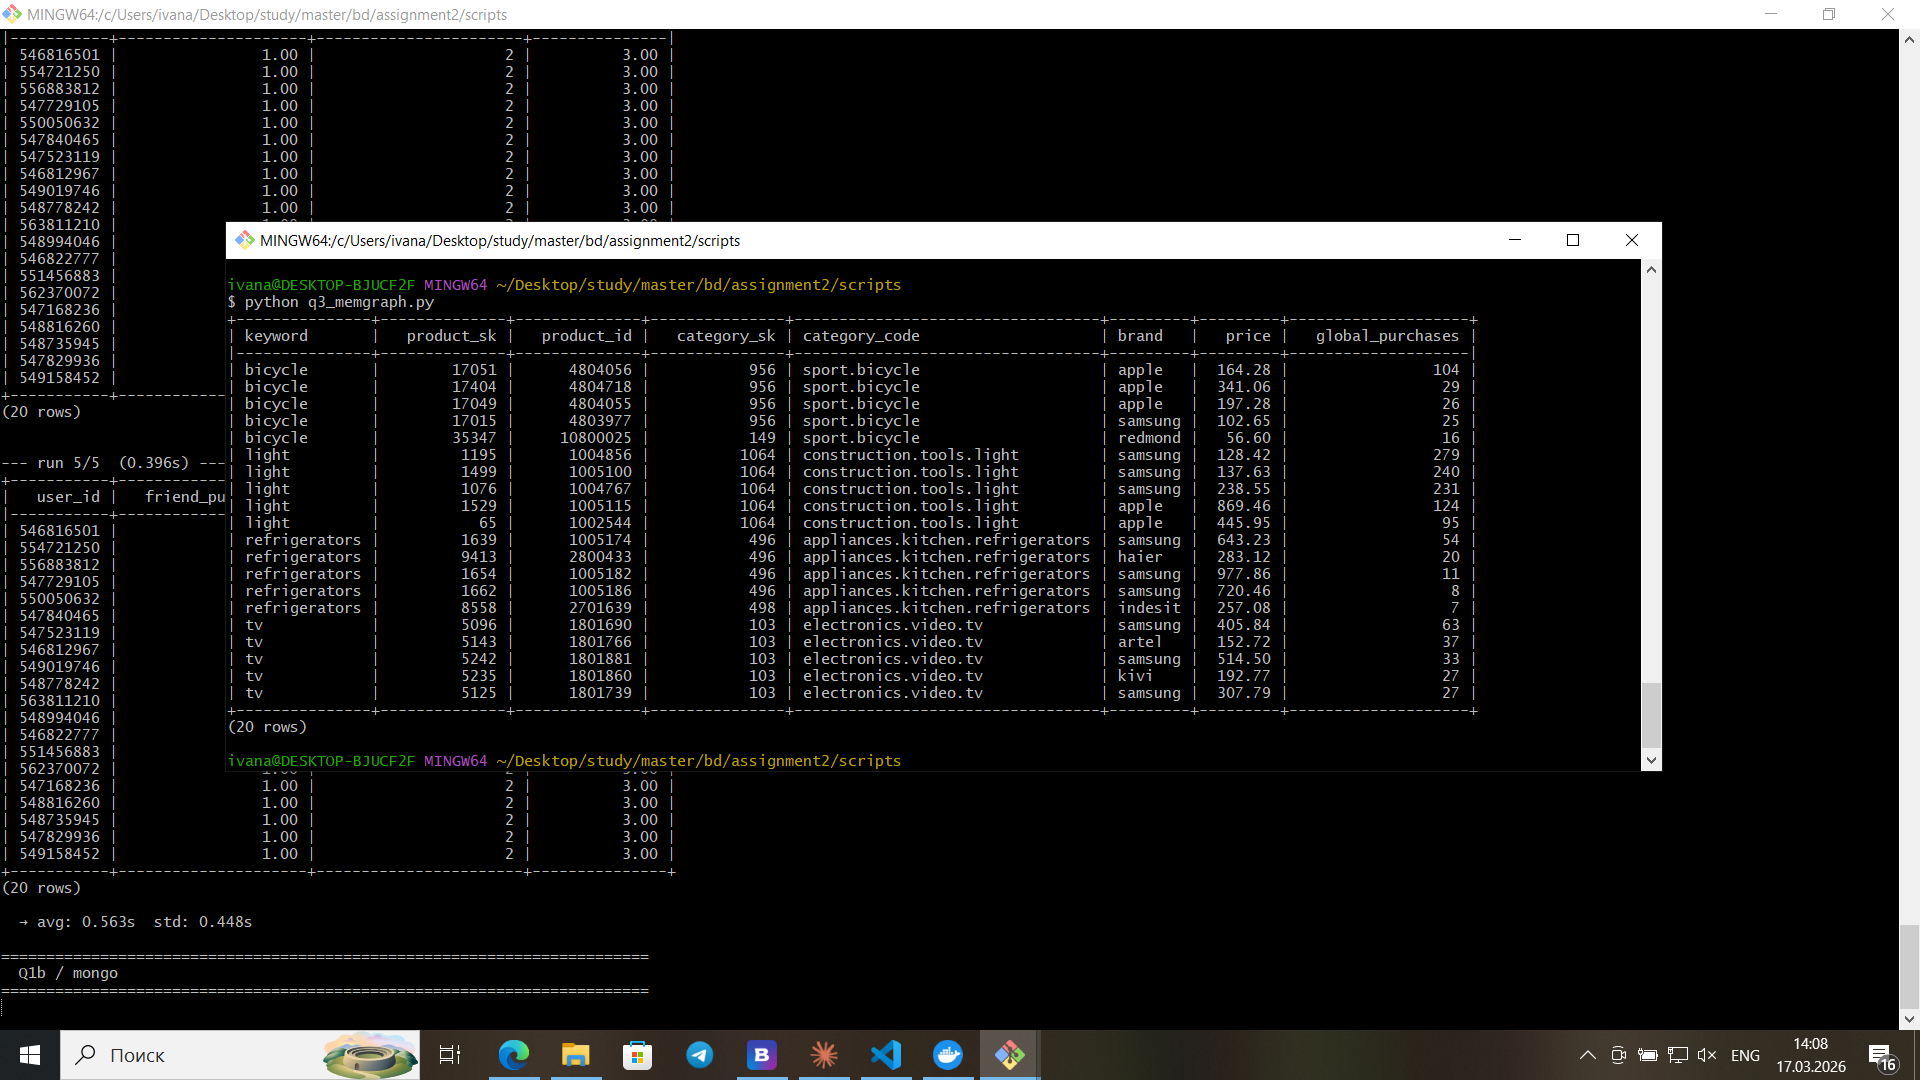
\includegraphics[width=\linewidth]{screenshots/q3_memgraph.png}
  \caption{Q3 results --- Memgraph}
\end{figure}

\textbf{Cross-query observation:} The Q3 results demonstrate that full-text
search integrates naturally with the recommendation engine from Q2. For
instance, user \texttt{546806144} has \texttt{construction.tools.light} among
their top preferred categories, with \texttt{product\_id=1004856} (Samsung)
as the top recommendation. A keyword search for ``light'' in Q3 surfaces
the same \texttt{product\_id=1004856} as the first result --- confirming
that the most globally popular product in a category is consistently
discoverable both through personalised recommendations and through
free-text search.

\subsection{Performance Summary}

Table~\ref{tab:bench} reports average and standard deviation of execution
times (wall-clock, including connection and pandas post-processing where
applicable) over 5 warm runs.

\begin{table}[H]
\centering
\small
\begin{tabular}{llrrrr}
\toprule
\textbf{Query} & \textbf{Metric} &
  \textbf{psql} & \textbf{psql\_own} & \textbf{MongoDB} & \textbf{Memgraph} \\
\midrule
\multirow{2}{*}{Q1a} & avg (s) & 0.83 & 0.90 & 3.57  & 6.13  \\
                     & std (s) & 0.03 & 0.10 & 0.26  & 0.14  \\
\midrule
\multirow{2}{*}{Q1b} & avg (s) & 0.47 & 0.40 & 1773.7 & 2.45  \\
                     & std (s) & 0.14 & 0.03 & 36.8   & 0.20  \\
\midrule
\multirow{2}{*}{Q2}  & avg (s) & 2.41 & 1.40 & 1773.3 & 396.3 \\
                     & std (s) & 0.18 & 0.14 & 21.8   & 0.99  \\
\midrule
\multirow{2}{*}{Q3}  & avg (s) & 0.51 & 0.61 & 2.37   & 1214.9 \\
                     & std (s) & 0.04 & 0.07 & 0.04   & 6.9   \\
\bottomrule
\end{tabular}
\caption{Benchmark results: avg $\pm$ std over 5 runs (seconds)}
\label{tab:bench}
\end{table}

\begin{figure}[H]
\centering
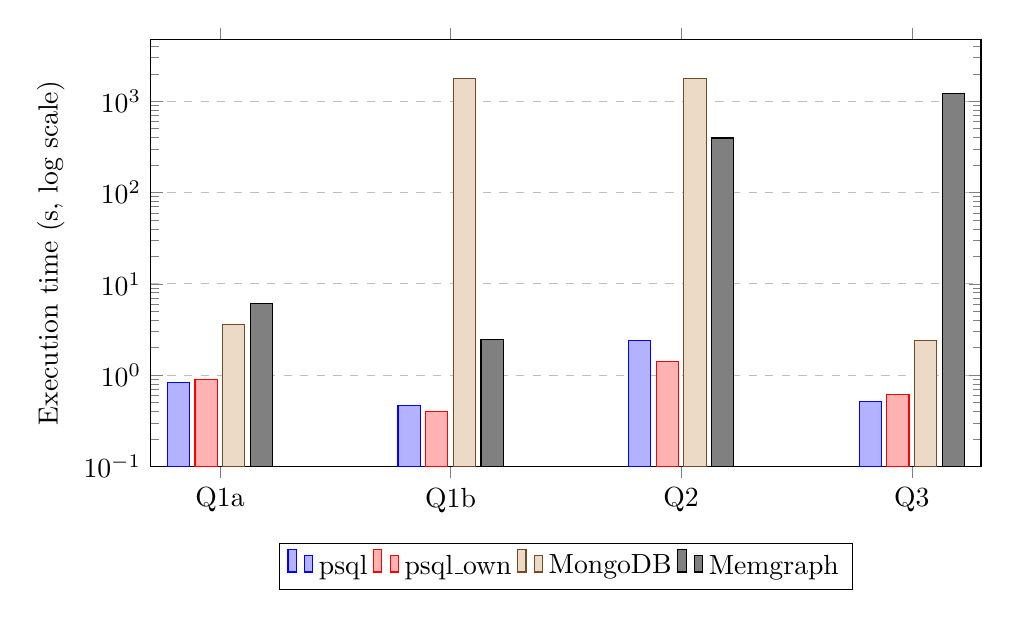
\begin{tikzpicture}
\begin{axis}[
  ybar,
  bar width=8pt,
  width=\linewidth,
  height=7cm,
  ymode=log,
  log origin=infty,
  ylabel={Execution time (s, log scale)},
  xtick=data,
  xticklabels={Q1a, Q1b, Q2, Q3},
  legend style={at={(0.5,-0.18)}, anchor=north, legend columns=4},
  ymajorgrids=true,
  grid style=dashed,
  ymin=0.1,
]
\addplot coordinates {(1,0.83)(2,0.47)(3,2.41)(4,0.51)};
\addplot coordinates {(1,0.90)(2,0.40)(3,1.40)(4,0.61)};
\addplot coordinates {(1,3.57)(2,1773.7)(3,1773.3)(4,2.37)};
\addplot coordinates {(1,6.13)(2,2.45)(3,396.3)(4,1214.9)};
\legend{psql, psql\_own, MongoDB, Memgraph}
\end{axis}
\end{tikzpicture}
\caption{Query execution times (logarithmic scale)}
\label{fig:chart}
\end{figure}

\begin{figure}[H]
  \centering
  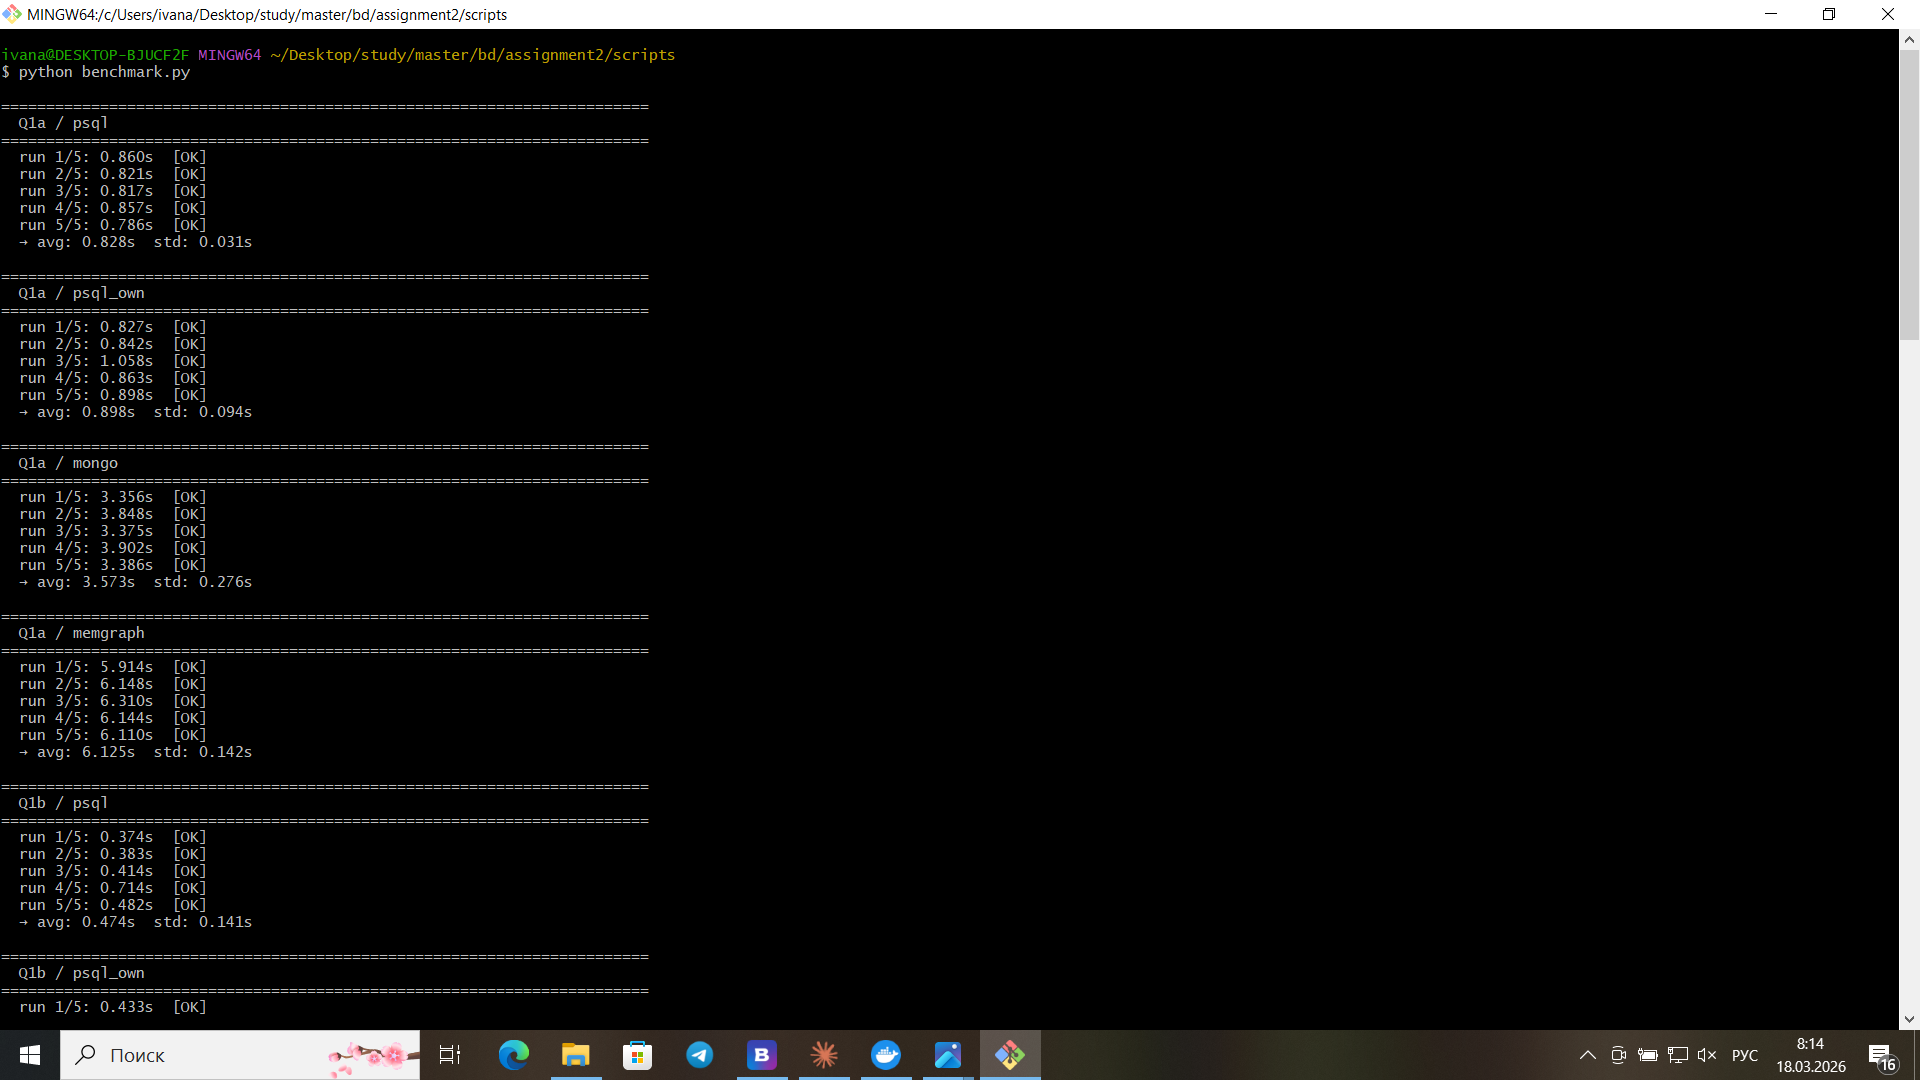
\includegraphics[width=\linewidth]{screenshots/benchmark (1).png}
  \caption{Benchmark terminal output (part 1)}
\end{figure}

\begin{figure}[H]
  \centering
  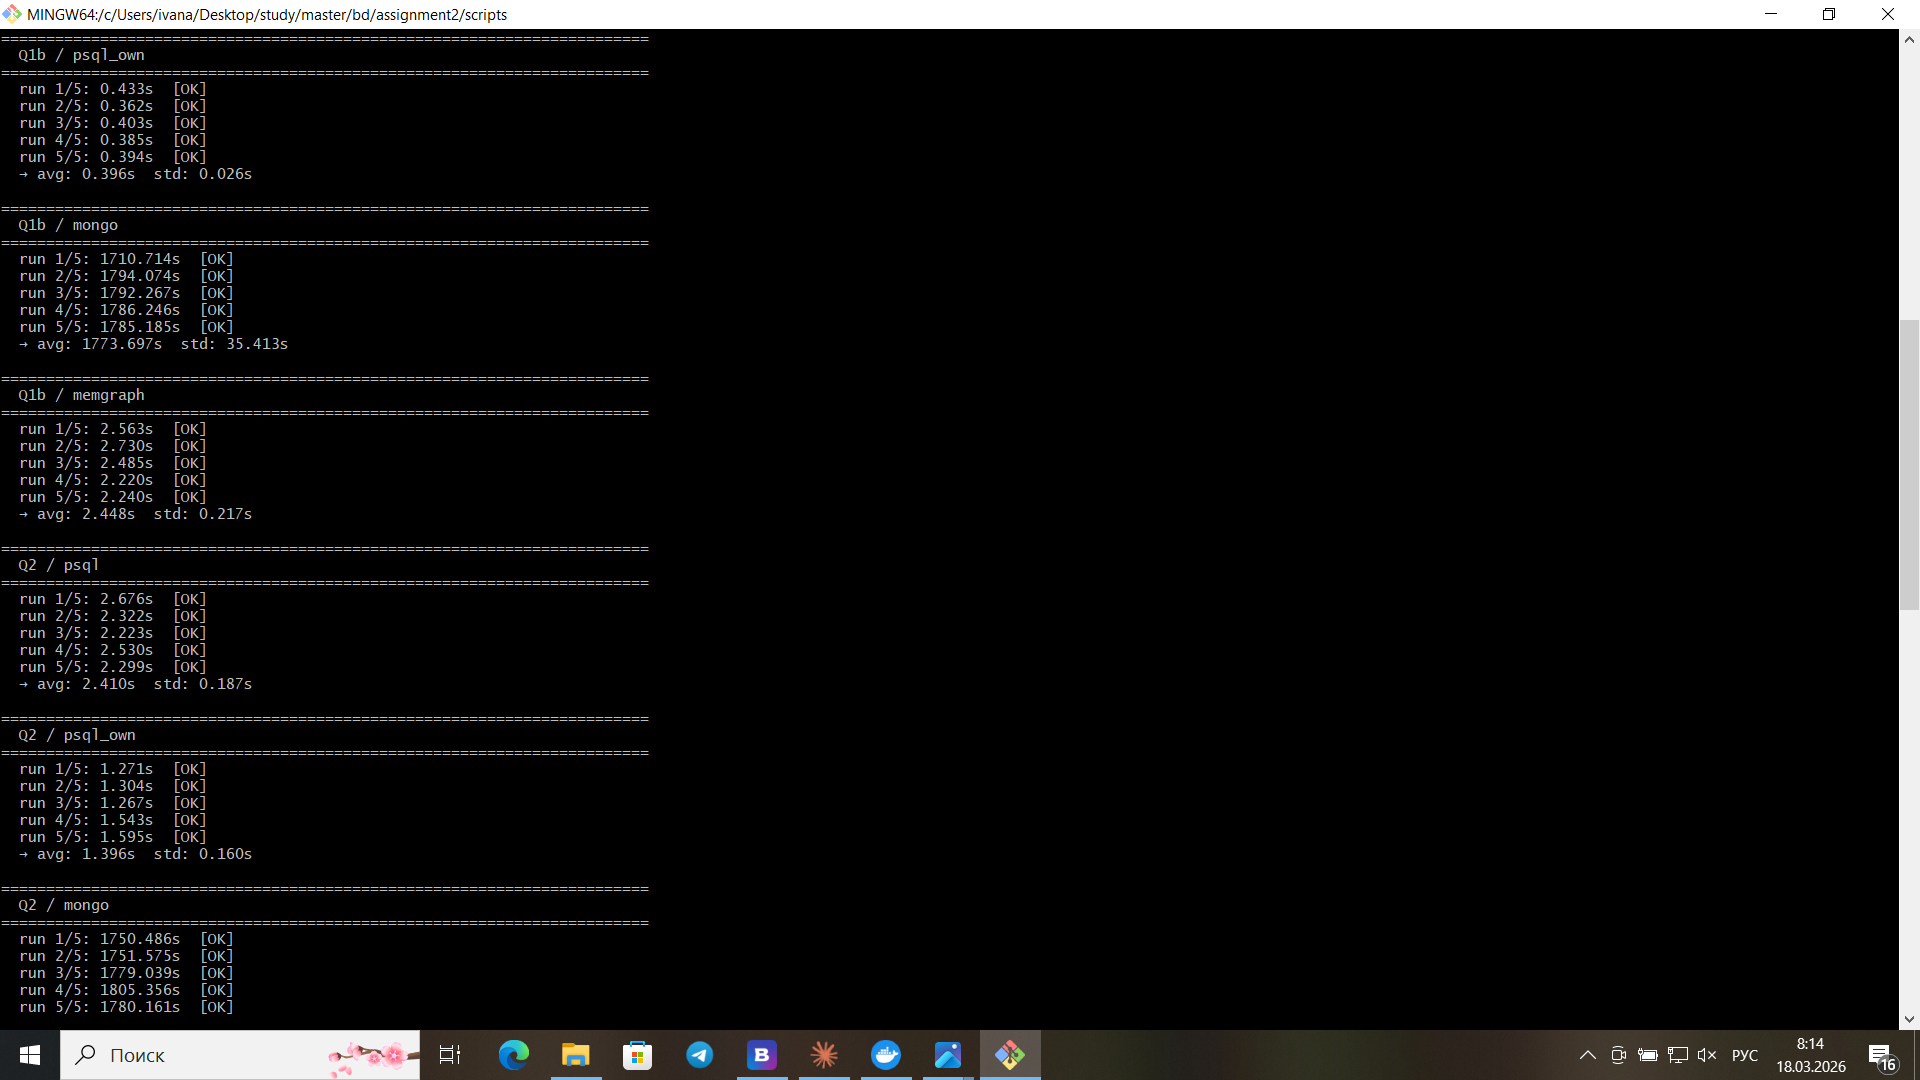
\includegraphics[width=\linewidth]{screenshots/benchmark (2).png}
  \caption{Benchmark terminal output (part 2)}
\end{figure}

\begin{figure}[H]
  \centering
  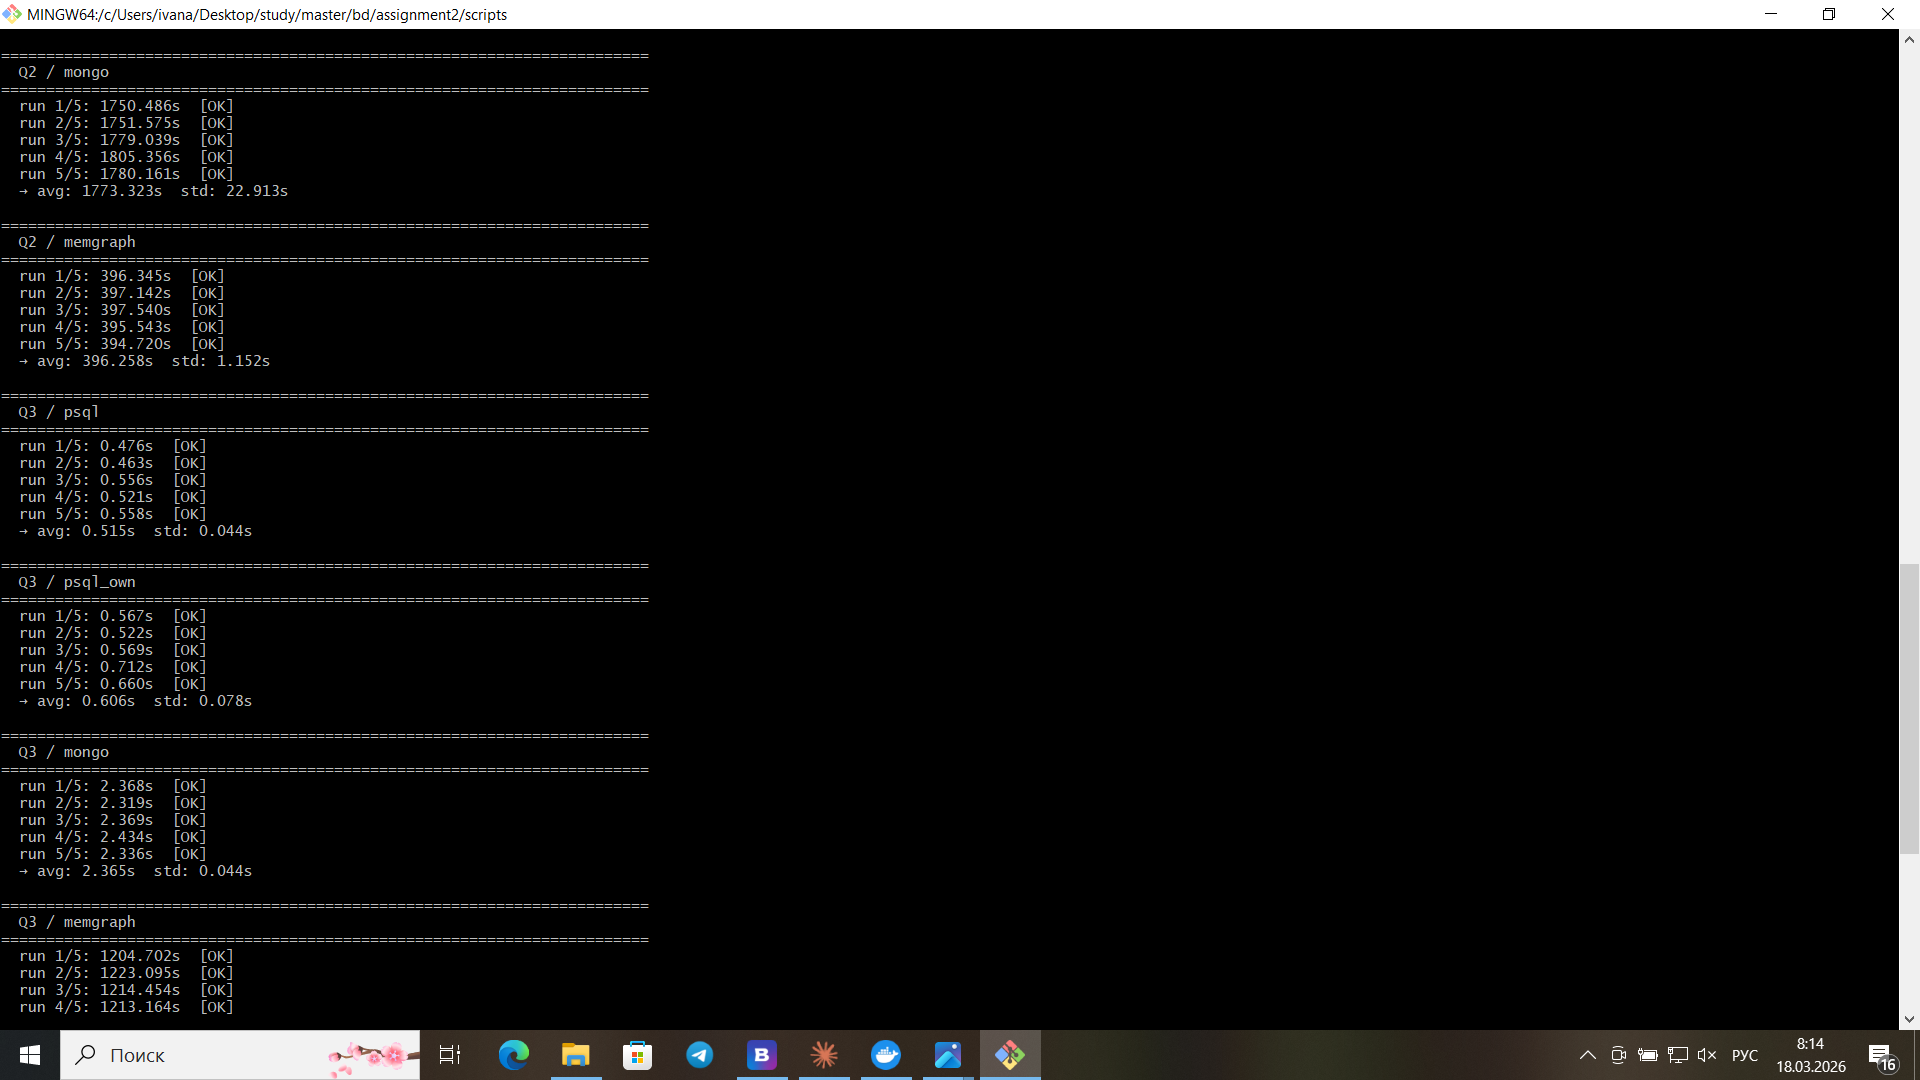
\includegraphics[width=\linewidth]{screenshots/benchmark (3).png}
  \caption{Benchmark terminal output (part 3)}
\end{figure}

\begin{figure}[H]
  \centering
  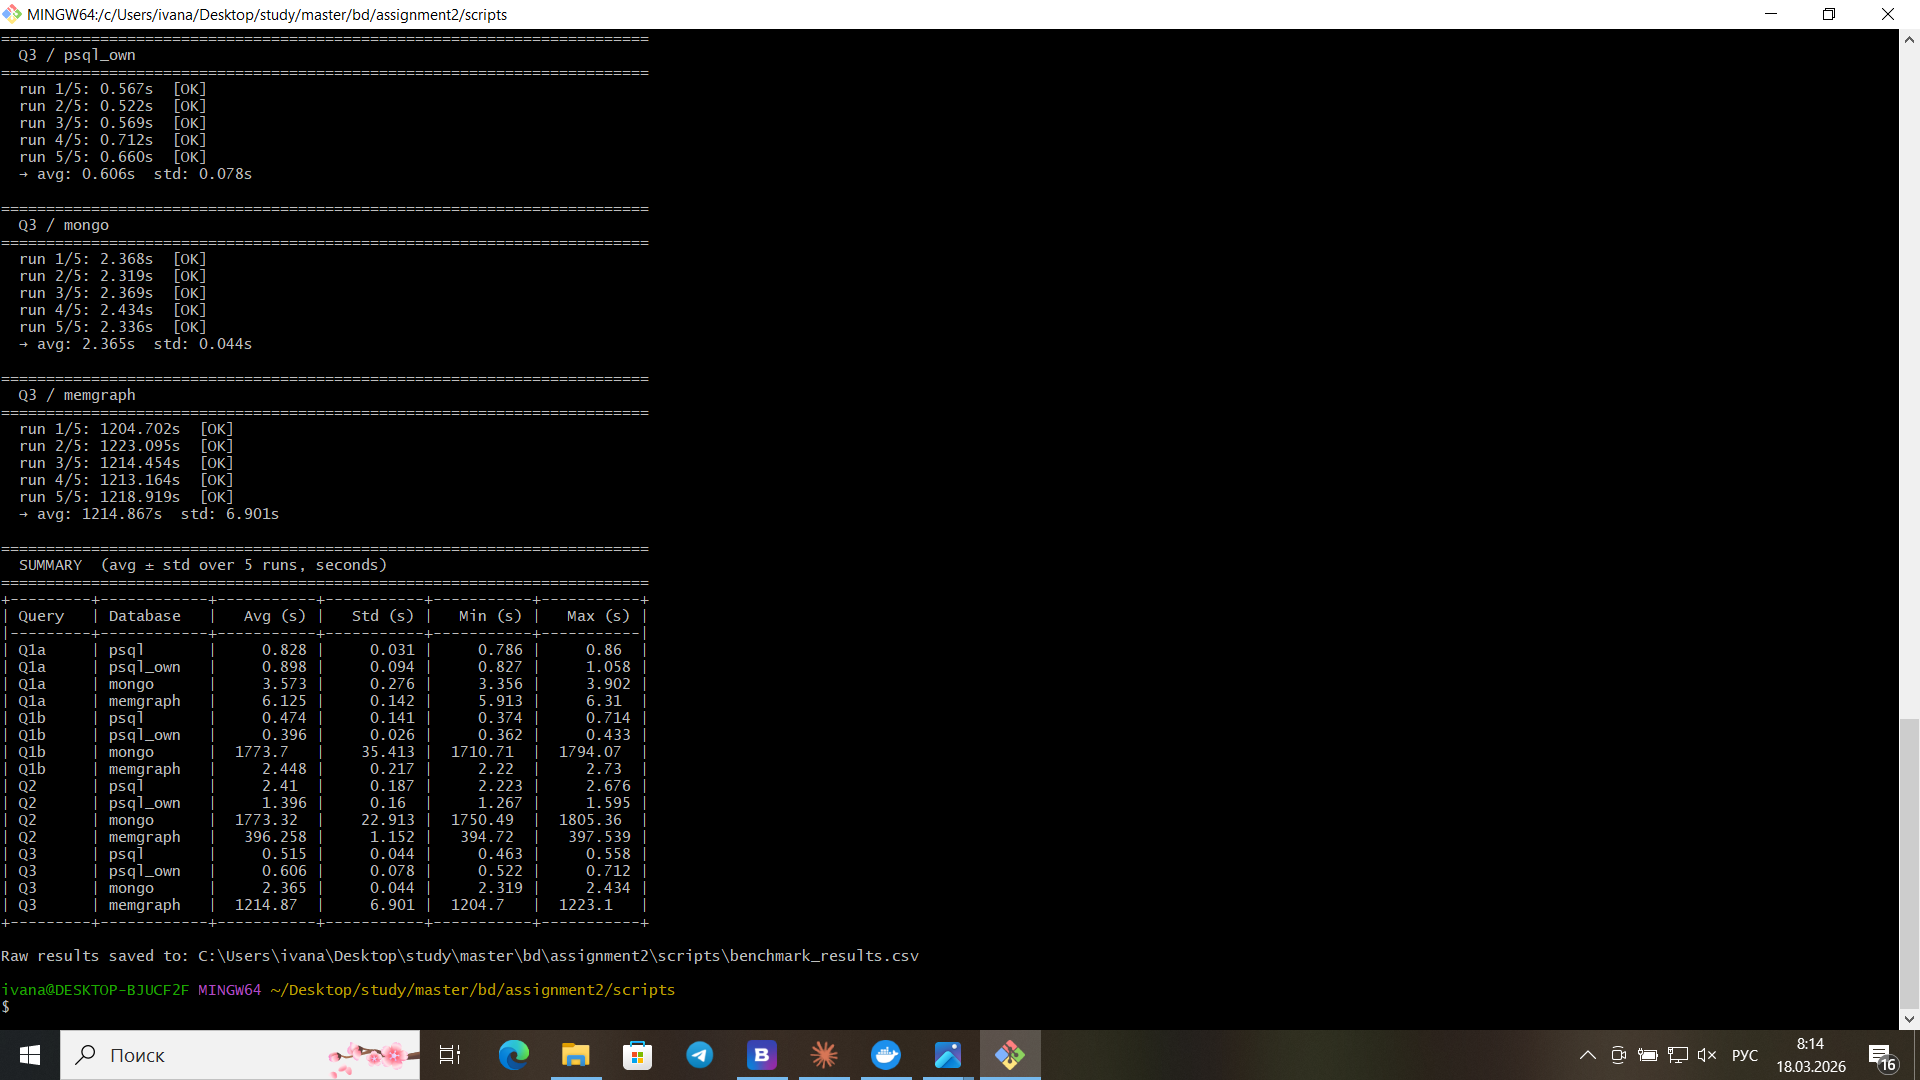
\includegraphics[width=\linewidth]{screenshots/benchmark (4).png}
  \caption{Benchmark terminal output (part 4)}
\end{figure}

% ═════════════════════════════════════════════════════════════════════════════
\section{Discussion}
% ═════════════════════════════════════════════════════════════════════════════

\subsection{PostgreSQL 3NF vs.\ Own Model}

The denormalised \emph{Own} model outperformed 3NF on Q2 ($1.40$ s vs.\ $2.41$ s,
a $\approx42\%$ speedup) by eliminating the join between \texttt{events} and
\texttt{products} for category resolution. For Q1a and Q1b, which do not
touch the product/category tables, the two models performed equivalently.
Q3 was marginally slower in the Own model because the larger \texttt{events}
table (with inline columns) slightly increases the cost of the
\texttt{global\_pop} aggregation.

These results confirm the classical trade-off: denormalisation benefits
\emph{read-heavy aggregation workloads} at the expense of storage and
write complexity.

\subsection{MongoDB}

MongoDB performed reasonably for simple aggregations (Q1a, Q3: 2--4 s) but
failed catastrophically for queries involving social graph traversal (Q1b:
$\approx$1774 s) and large correlated aggregations (Q2: $\approx$1773 s).

The root cause in both cases is the same: MongoDB's aggregation pipeline
executes \texttt{\$lookup} as a \emph{nested-loop join}. For Q1b, each
user requires a full scan of the \texttt{friendships} collection to find
friends, then another scan of \texttt{messages} to check purchases. For Q2,
the original correlated pipeline performed a full \texttt{events} scan per
(user, category) pair. Splitting Q2 into four independent pipelines and
finishing with pandas reduced the algorithmic complexity from $O(N_u \cdot
N_c \cdot N_e)$ to $O(N_e)$, yet the runtime remained high because three
out of four pipelines still scan the full events collection.

\subsection{Memgraph}

Memgraph delivered its best result on Q1b ($2.45$ s), where the native graph
traversal (\texttt{FRIENDS\_WITH} + \texttt{RECEIVED} pattern matching)
processes the social network efficiently. This is the workload graph databases
are designed for.

However, Memgraph struggled severely with global aggregations:
\begin{itemize}
  \item \textbf{Q2 (396 s):} Counting all purchase events per product across
        the entire graph requires scanning all \texttt{HAD\_EVENT} edges.
        Unlike an RDBMS with a columnar index on \texttt{event\_type}, Memgraph
        traverses adjacency lists, which are optimised for pattern matching,
        not column scans.
  \item \textbf{Q3 (1215 s):} The same global purchase count computed per
        candidate product inside a list comprehension creates quadratic
        complexity when many products match the search keywords.
\end{itemize}

\subsection{Result Consistency}

All four databases produced \textbf{identical results} for Q1a, Q1b, and Q3.
For Q2, PostgreSQL 3NF and Own, and Memgraph produced identical output.
MongoDB Q2 results matched after the NaN-handling fix for products with
missing category codes was applied. The consistency confirms that the
SCD~Type~2 surrogate key design achieved its goal: every model resolves the
historically correct category for each event.

\subsection{Summary of Strengths and Weaknesses}

\begin{table}[H]
\centering
\small
\begin{tabularx}{\linewidth}{lXX}
\toprule
\textbf{Database} & \textbf{Strengths} & \textbf{Weaknesses} \\
\midrule
PostgreSQL 3NF &
  Fast aggregations; ACID; mature query optimiser; index support for all join patterns &
  Multi-table joins for every query; no native graph traversal \\
\midrule
PostgreSQL Own &
  Fastest Q2 (inline columns); same ACID guarantees; simple queries &
  Update anomalies; higher storage; schema redundancy \\
\midrule
MongoDB &
  Schema flexibility; simple queries fast; horizontal scaling potential &
  Correlated \texttt{\$lookup} extremely slow; no efficient graph traversal; no joins by design \\
\midrule
Memgraph &
  Excellent for social/graph queries (Q1b); expressive Cypher for patterns &
  Slow global aggregations; high memory use; no columnar scan optimisations \\
\bottomrule
\end{tabularx}
\caption{Summary of database model characteristics}
\end{table}

\textbf{Conclusion:} For this mixed workload (marketing analytics + social
scoring + recommendations + search), PostgreSQL with appropriate denormalisation
provides the best overall performance. Memgraph is a strong complement for
the social-graph query specifically, where its native traversal outperforms
all other models. MongoDB performs well for simple aggregations but requires
careful pipeline design to avoid the nested-loop join behaviour of
\texttt{\$lookup}, which becomes prohibitive for large collections.

\end{document}
